% !TEX spellcheck = nl_NL
\documentclass[a4paper]{report}
\usepackage{graphicx}
\usepackage{todonotes}
\usepackage[dutch]{babel} 
\usepackage{enumerate}
\usepackage[utf8]{inputenc} % Set input to UTF-8 to enable easy input of umlauts etc.
\usepackage{hyperref} % Turn references into links.
\usepackage[hypcap]{caption} % Make figure references point to top of figure.
\usepackage{listings} % listings to include code samples
\usepackage{xspace} % Keeps space after lstinline commands.
\usepackage{caption}
\usepackage{xcolor} % to change color in code listings
\usepackage[T1]{fontenc}  
\usepackage{textcomp}  
\usepackage{lmodern}  
\usepackage{float}
\usepackage{multirow}
\usepackage{enumitem}
\usepackage{tabularx}
\usepackage{qtree}
\usepackage{etoolbox}
\usepackage{newfloat} %used to draw trees (qtree) in a floating enviroment for captions
\usepackage[a4paper]{geometry}
\providetoggle{longTests}
\DeclareFloatingEnvironment[fileext=lod]{diagram} %create a floating enviroment for qtree

\usepackage{pdflscape}
\DeclareCaptionFont{white}{ \color{white} }
\DeclareCaptionFormat{listing}{
  \colorbox[cmyk]{0.43, 0.35, 0.35,0.01 }{
    \parbox{\textwidth}{\hspace{15pt}#1#2#3}
  }
}
\captionsetup[lstlisting]{ format=listing, labelfont=white, textfont=white, singlelinecheck=false, margin=0pt, font={bf,footnotesize} }

%hyphenation
\hyphenation{back-logs}

% set parameters for lstlisting and lstinline
\lstset{
  breaklines=true, % Enables wrapping in lstlisting environment.
  backgroundcolor=\color[HTML]{F8F8F8},
  frame=tlrb,
  basicstyle=\ttfamily, % the size of the fonts that are used for the code
  keepspaces=true, 
  language=Haskell,
  framextopmargin=5pt,
  framexleftmargin=5pt,
  framexrightmargin=5pt,
  framexbottommargin=5pt,
  commentstyle=\itshape\color[HTML]{999988},
  rulecolor=\color[HTML]{DDDDDD},
  stringstyle=\color[HTML]{dd1144},
  keywordstyle=\idstyle,
  identifierstyle=\idstyle,
  keywords={as, case, of, class, data, data family, data instance, default, deriving, deriving instance, do, forall, foreign, hiding, if, then, else, import, infix, infixl, infixr, instance, let, in, mdo, module, newtype, proc, qualified, rec, type, type family, type instance, where},
  keywordstyle=\color[HTML]{333333}\bfseries, 
  numbers=left, %we need line numbers to make line wrapping obvious
  numberstyle=\color[HTML]{888888}, %we want line numbers to blend in
  tabsize=4,
  literate={ö}{{\"o}}1 %handle some special chars
           {ä}{{\"a}}1
           {ü}{{\"u}}1
           {ë}{{\"e}}1
           {ï}{{\"i}}1
           {0}{{{\color[HTML]{009999}{0}}}}{1}
           {1}{{{\color[HTML]{009999}{1}}}}{1}
           {2}{{{\color[HTML]{009999}{2}}}}{1}
           {3}{{{\color[HTML]{009999}{3}}}}{1}
           {4}{{{\color[HTML]{009999}{4}}}}{1}
           {5}{{{\color[HTML]{009999}{5}}}}{1}
           {6}{{{\color[HTML]{009999}{6}}}}{1}
           {7}{{{\color[HTML]{009999}{7}}}}{1}
           {8}{{{\color[HTML]{009999}{8}}}}{1}
           {9}{{{\color[HTML]{009999}{9}}}}{1}
           {.0}{{{\color[HTML]{009999}{.0}}}}{1}
           {.1}{{{\color[HTML]{009999}{.1}}}}{1}
           {.2}{{{\color[HTML]{009999}{.2}}}}{1}
           {.3}{{{\color[HTML]{009999}{.3}}}}{1}
           {.4}{{{\color[HTML]{009999}{.4}}}}{1}
           {.5}{{{\color[HTML]{009999}{.5}}}}{1}
           {.6}{{{\color[HTML]{009999}{.6}}}}{1}
           {.7}{{{\color[HTML]{009999}{.7}}}}{1}
           {.8}{{{\color[HTML]{009999}{.8}}}}{1}
           {.9}{{{\color[HTML]{009999}{.9}}}}{1}
           {"}{\textquotedbl}1
           {'}{\textquotesingle}1
}
  % Use this to fit more code in the block
\lstdefinestyle{densecode}{
  aboveskip=1cm,
  belowskip=1cm,
  xleftmargin=-1.85cm, % Alters margin for listings to fit more code on a line.
  xrightmargin=-1.85cm, % Alters margin for listings to fit more code on a line.
  basicstyle=\small\ttfamily
}

\definecolor{lightgray}{rgb}{.9,.9,.9}
\definecolor{darkgray}{rgb}{.4,.4,.4}
\definecolor{purple}{rgb}{0.65, 0.12, 0.82}

\lstdefinelanguage{JavaScript}{
  keywords={typeof, new, true, false, catch, function, return, null, catch, switch, var, if, in, while, do, else, case, break},
  keywordstyle=\color{blue}\bfseries,
  ndkeywords={class, export, boolean, throw, implements, import, this},
  ndkeywordstyle=\color{darkgray}\bfseries,
  identifierstyle=\color{black},
  sensitive=false,
  comment=[l]{//},
  tabsize=2,
  morecomment=[s]{/*}{*/},
  commentstyle=\color{purple}\ttfamily,
  stringstyle=\color{red}\ttfamily,
  morestring=[b]',
  morestring=[b]"
}
\renewcommand{\lstlistingname}{Code}

\makeatletter
\newcommand*\idstyle{%
        \expandafter\id@style\the\lst@token\relax
}
\def\id@style#1#2\relax{%
        \ifcat#1\relax\else
                \ifnum`#1=\uccode`#1%
                        \color[HTML]{445588}\bfseries
                \else
                        \color[HTML]{333333}\normalfont
                \fi
        \fi
}
\makeatother
% command to properly show inline code
\newcommand{\inlinecode}[1]{\lstinline[basicstyle=\ttfamily,keywordstyle=\bfseries,identifierstyle=\bfseries,stringstyle=\bfseries,literate={}]|#1|}
\newcommand{\inlinecodequotes}{\lstinline[basicstyle=\ttfamily,keywordstyle=\bfseries,identifierstyle=\bfseries,literate={}]} %If it starts with quotes it otherwise doesn't work

% Necessary to make \autoref command display nice Dutch words.
  \def\equationautorefname{Vergelijking}
  \def\footnoteautorefname{voetnoot}
  \def\itemautorefname{item}
  \def\figureautorefname{Figuur}
  \def\tableautorefname{Tabel}
  \def\partautorefname{Deel}
  \def\appendixautorefname{Appendix}
  \def\chapterautorefname{Hoofdstuk}
  \def\sectionautorefname{sectie}
  \def\subsectionautorefname{subsectie}
  \def\subsubsectionautorefname{subsubsectie}
  \def\paragraphautorefname{paragraaf}
  \def\subparagraphautorefname{subparagraaf}
  \def\FancyVerbLineautorefname{regel}
  \def\theoremautorefname{Theorema}
  \def\pageautorefname{pagina}

% Two new commands to display references a certain way.
\newcommand*{\fullref}[1]{\hyperref[{#1}]{\autoref*{#1}} \nameref*{#1}}
\newcommand*{\halfref}[1]{\hyperref[{#1}]{\ref*{#1}} \nameref*{#1}}

\makeindex
\geometry{a4paper,textwidth=345pt,textheight=598pt}
\begin{document}
\begin{titlepage}

\newcommand{\HRule}{\rule{\linewidth}{0.5mm}} % Defines a new command for the horizontal lines, change thickness here

\center % Center everything on the page
\vspace*{\fill}
 
%----------------------------------------------------------------------------------------
%	HEADING SECTIONS
%----------------------------------------------------------------------------------------

\textsc{\LARGE Universiteit Twente}\\[1.5cm] % Name of your university/college
\textsc{\Large Ontwerpproject}\\[2.0cm] % Major heading such as course name
%\textsc{\large Minor Heading}\\[0.5cm] % Minor heading such as course title

%----------------------------------------------------------------------------------------
%	TITLE SECTION
%----------------------------------------------------------------------------------------

\HRule \\[0.6cm]
{ \huge \bfseries Canvas.hs}\\[0.4cm] % Title of your document
{ \large \bfseries Event driven I/O voor Haskell met het HTML canvas}\\[0.4cm] % Title of your document
\HRule \\[1.8cm]
 
%----------------------------------------------------------------------------------------
%	AUTHOR SECTION
%----------------------------------------------------------------------------------------

\begin{minipage}[t]{0.4\textwidth}
\begin{flushleft} \large
\emph{Auteurs:}\\
J. \textsc{van Doorn}\\
L.J. \textsc{Buit}\\
P.T. \textsc{Jager}\\
M.J. \textsc{Scheepers}\\
M.J. \textsc{Roo}
\end{flushleft}
\end{minipage}
~
\begin{minipage}[t]{0.4\textwidth}
\begin{flushright} \large
\emph{Begeleider:} \\
E. \textsc{de Groote}
\end{flushright}
\end{minipage}\\[4cm]

% If you don't want a supervisor, uncomment the two lines below and remove the section above
%\Large \emph{Author:}\\
%John \textsc{Smith}\\[3cm] % Your name

%----------------------------------------------------------------------------------------
%	DATE SECTION
%----------------------------------------------------------------------------------------

\vspace*{\fill}
{\large \today} % Date, change the \today to a set date if you want to be precise

%----------------------------------------------------------------------------------------
%	LOGO SECTION
%----------------------------------------------------------------------------------------

%\includegraphics{Logo}\\[1cm] % Include a department/university logo - this will require the graphicx package
 
%----------------------------------------------------------------------------------------


\end{titlepage}
\tableofcontents

% !TEX spellcheck = nl_NL
\chapter{Inleiding}
Bij het informatica-keuzevak Functioneel Programmeren gebruiken studenten Haskell om fundamentele concepten van functioneel programmeren te bestuderen. Hierbij wordt door de studenten veel gebruik gemaakt van grafische weergaven om de werking van hun code inzichtelijk te maken. Het gebruik van Haskell voor het maken van grafische weergaven blijkt vaak redelijk gecompliceerd en limiteert studenten doordat zij zich bezig moeten houden met minder intuïtieve en minder essentiële aspecten van Haskell.

Om de focus binnen Functioneel Programmeren op de essentie te houden, is een grafische omgeving ontwikkeld op basis van de Gloss grafische bibliotheek. De interface tussen de code van de student en de grafische interface is eenvoudig en bruikbaar, het bevat alleen een aantal nadelen. Het werkt niet goed op ieder platform, mist een aantal functionaliteiten en de prestatie is niet uitstekend.

In dit ontwerpproject is \emph{Canvas.hs} ontwikkeld; een omgeving die Haskell-gebruikers in staat stelt op eenvoudige wijze grafische elementen op een HTML5 canvas te presenteren. Canvas.hs is ontwikkeld met het oog op gebruiksgemak en eenvoud zonder de mogelijkheid tot uitbreiding en het toevoegen van geavanceerde functionaliteit onnodig te beperken.

\todo{uitbreiden met grove structuur van het project}

\subsubsection{Verslagstructuur}
In dit verslag wordt in \autoref{hoofdstuk:requirements} de requirements beschreven. In  \autoref{hoofdstuk:ontwerp} wordt het ontwerp van Canvas.hs beschreven. Dit hoofdstuk is onderverdeeld in de secties: \halfref{sec:globaal}, \halfref{sec:detail}, \halfref{sec:testplan} en \halfref{sec:testresultaten}. \autoref{hoofdstuk:conclusie} beschrijft de conclusies van dit project en in \autoref{hoofdstuk:evaluatie} wordt dit project met zijn uitkomsten geëvalueerd. Vervolgens wordt in \fullref{sec:gebruikershandleiding} een handleiding gepresenteerd die gebruikers van Canvas.hs aanwijzingen geeft over hoe de omgeving gebruikt en uitgebreid kan worden.



% !TEX spellcheck = nl_NL
\chapter{Organisatie}

Tijdens het ontwikkelen van de eerste versie van Canvas.hs is er samengewerkt volgens een paar vooraf geselecteerde methoden. Zo zijn er onderdelen van de Scrum projectmanagement methode toegepast voor een goede planning en duidelijke afspraken. Lees hier meer over in de volgende sectie—\halfref{sec:scrum}.

Bij het ontwikkelen van software is het naast een goede project organisatie ook zaak dat er door ontwikkelaars goed samengewerkt kan worden op technisch vlak. Daarbij is het elkaar controlleren en elkaar niet in de weg zitten een belangrijk onderdeel. Hoe dit tijdens de ontwikkeling van Canvas.hs georganiseerd is kan gelezen worden in \fullref{sec:technische_organisatie}.

\section{Scrum} \label{sec:scrum}

Er is gewerkt middels de scrum projectmangement methoden. Er is gewerkt met verschillende rollen en er zijn zogenaamde scrum en sprint besprekingen gehouden. Daarbij zijn elke keer opnieuw onder andere het project– en sprintbacklog samengesteld en bijgewerkt.

\paragraph{Rollen} Er is een verdeling van verantwoordelijkheden gemaakt. Naast de teamleden nam de opdrachtgever de rol van \emph{product owner} aan.
\begin{enumerate}
    \item \emph{J. van Doorn} had de taak van \emph{scrum master} en was verantwoordelijk voor het testen van de software.
    \item \emph{P.T. Jager} was notulist voor alle besprekingen en samen met Buit verantwoordelijk voor de Haskell code.
    \item \emph{L.J. Buit} was verantwoordelijk voor het protocol en samen met Jager verantwoordelijk voor de Haskell code.
    \item \emph{M.J. Roo} was samen met Scheepers verantwoordelijk voor de JavaScript code.
    \item \emph{M.J. Scheepers} was verantwoordelijk voor de gebruiksvriendelijkheid uiteindelijke API en samen met Roo verantwoordelijk voor de JavaScript code.
\end{enumerate}

\paragraph{Besprekingen} Elke samenkomst is er een kortdurende scrumbespreking gehouden. Na aanvang van het project zijn er ook een aantal sprint besprekingen gehouden. Deze sprint besprekingen kwamen altijd na het gesprek met de opdrachtgever. Er bleek al snel dat onze afgesproken sprint van twee werken wel erg kort was om elke twee weken dat er samengekomen werd een nieuwe lange sprintbespreking te houden. Dus er werd uiteindelijk voor gekozen om de besprekingen met de projectgroep te beperkingen tot de dagelijkse korte besprekingen.

Bij de dagelijkse besprekingen werd vaak op details in gegaan, hierbij werden ontwerp beslissingen vaak genomen tijdens deze besprekingen. De besprekingen duurde hierdoor soms wat lang en werden zittend gehouden.

\paragraph{Taken}
Regelmatig werd de lijst met taken bijgewerkt. Taken bestonden uit: projecttaken, als het bijhouden van de planning; ontwikkeltaken, als het oplossen van bugs en het schrijven van nieuwe features; schrijftaken en overige taken.

\begin{figure}[H]
\begin{center}
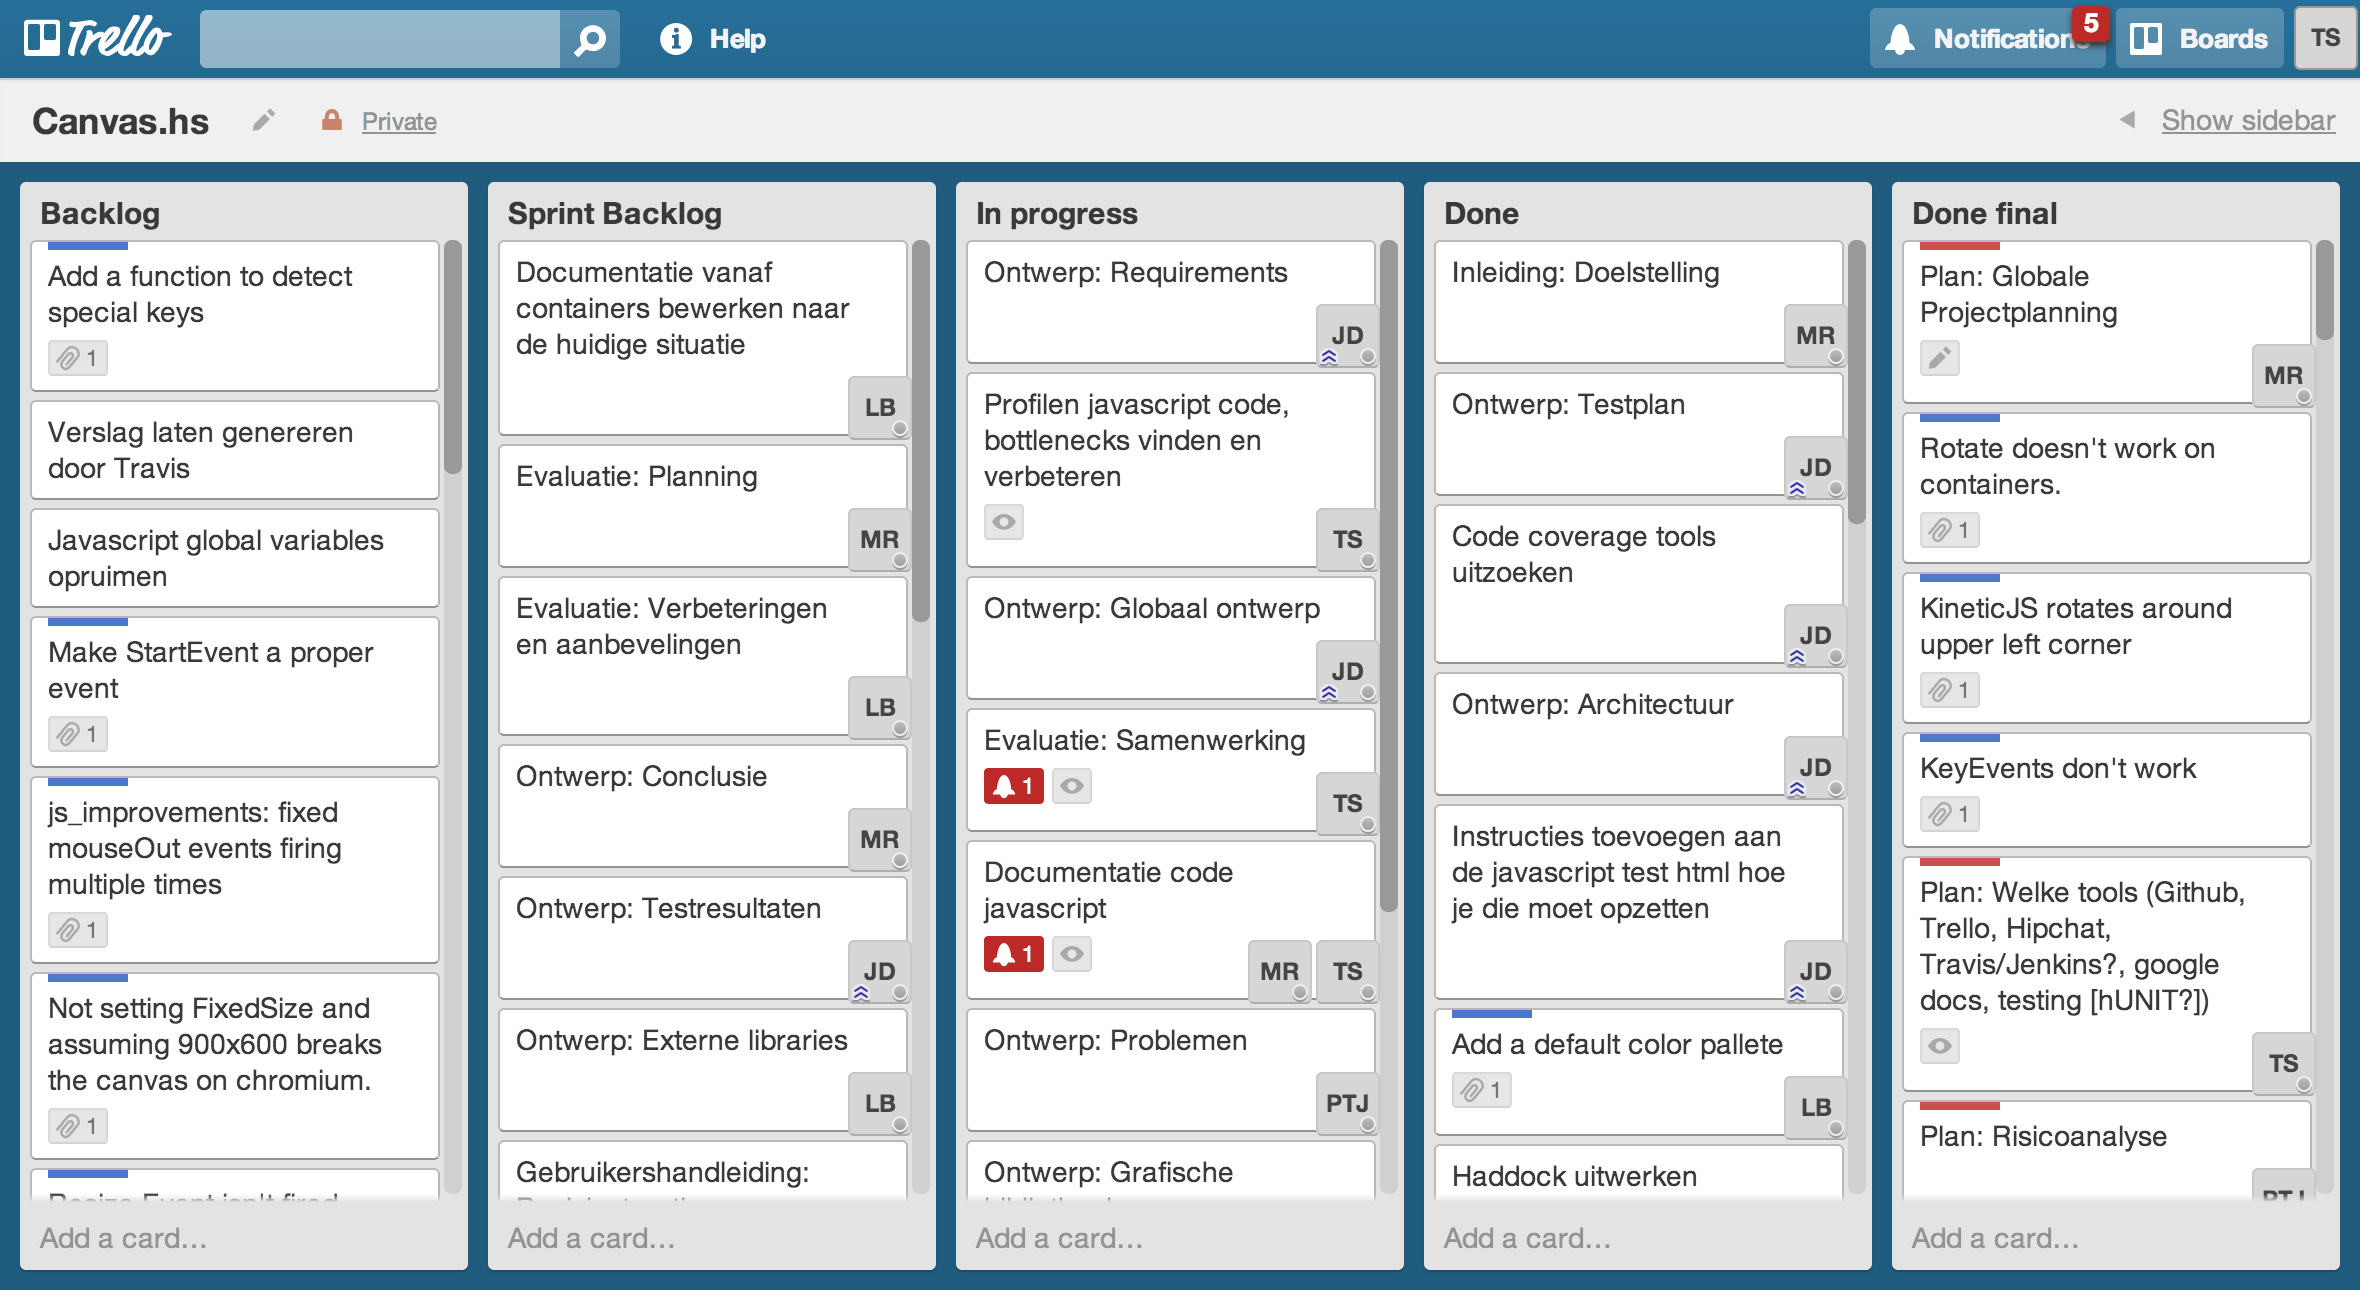
\includegraphics[keepaspectratio,width=\textwidth]{./images/trello.png}
\caption{Trello board}
\label{fig:trello}
\end{center}
\end{figure}

De lijst van ontwikkeltaken werd bijgehouden op het \emph{GitHub} platform. Deze taken werden daar ook wel Issues genoemd. Andere taken werden vervolgens bijgehouden op \emph{Trello}. Met deze applicatie kan een online takenbord gemaakt worden, zie \autoref{fig:trello}. De ontwikkeltaken werden middels synchronisatie ook op dit takenbord gezet. Door \emph{Trello} had elk lid van het project een goed inzicht in de taken die nog openstonden en reeds waren uitgevoerd.

\paragraph{Terugkoppeling naar de opdrachtgever} De opdrachtgever—binnen scrum ook \emph{product owner} genoemd—is twee wekelijks ge\"informeerd over de voortgang. De terugkoppeling die de opdrachtgever gaf werd besproken en verwerkt in de volgende versie van de library.

\subsection{Terugkoppeling}

\section{Technische organisatie}  \label{sec:technische_organisatie}
Bij het bouwen van software met een groep is het belangrijk dat een ontwikkelaar zich kan concentreren op de feature die hij aan het ontwikkelen is. Idealiter hoeft er geen rekening gehouden te worden met andere features die door anderen ontwikkeld worden. Er is dan ook gekozen om gebruik te maken van het gedistribueerde versiebeheer systeem \emph{Git} met een centraal repository op \emph{GitHub}.

Over het gebruik van deze software zijn afspraken gemaakt. Zo is er gebruik gemaakt van verschillende \emph{branches}. Als een bepaalde versie van de software op een bepaalde branch staat zegt dit iets over de status van die versie. Zo kan er begonnen worden aan een nieuwe feature vanaf de \inlinecode{dev} branch. En is een versie op de \inlinecode{master} branch klaar voor gebruik.

\subsection{Gitflow en pull requests}

Bij aanvang van de ontwikkeling van een nieuwe feature werd er een nieuwe branch gemaakt vanaf de \inlinecode{dev} branch. Een voorbeeld hiervan is de \inlinecode{arcs} branch. In \autoref{sec:shapesext} staat beschreven hoe \inlinecode{Arc} shapes toegevoegd kunnen worden. Dit is dus gebeurd op een aparte branch die begonnen is vanaf de \inlinecode{dev} branch, zie \autoref{fig:pullrequest}. 

\begin{figure}
\begin{center}
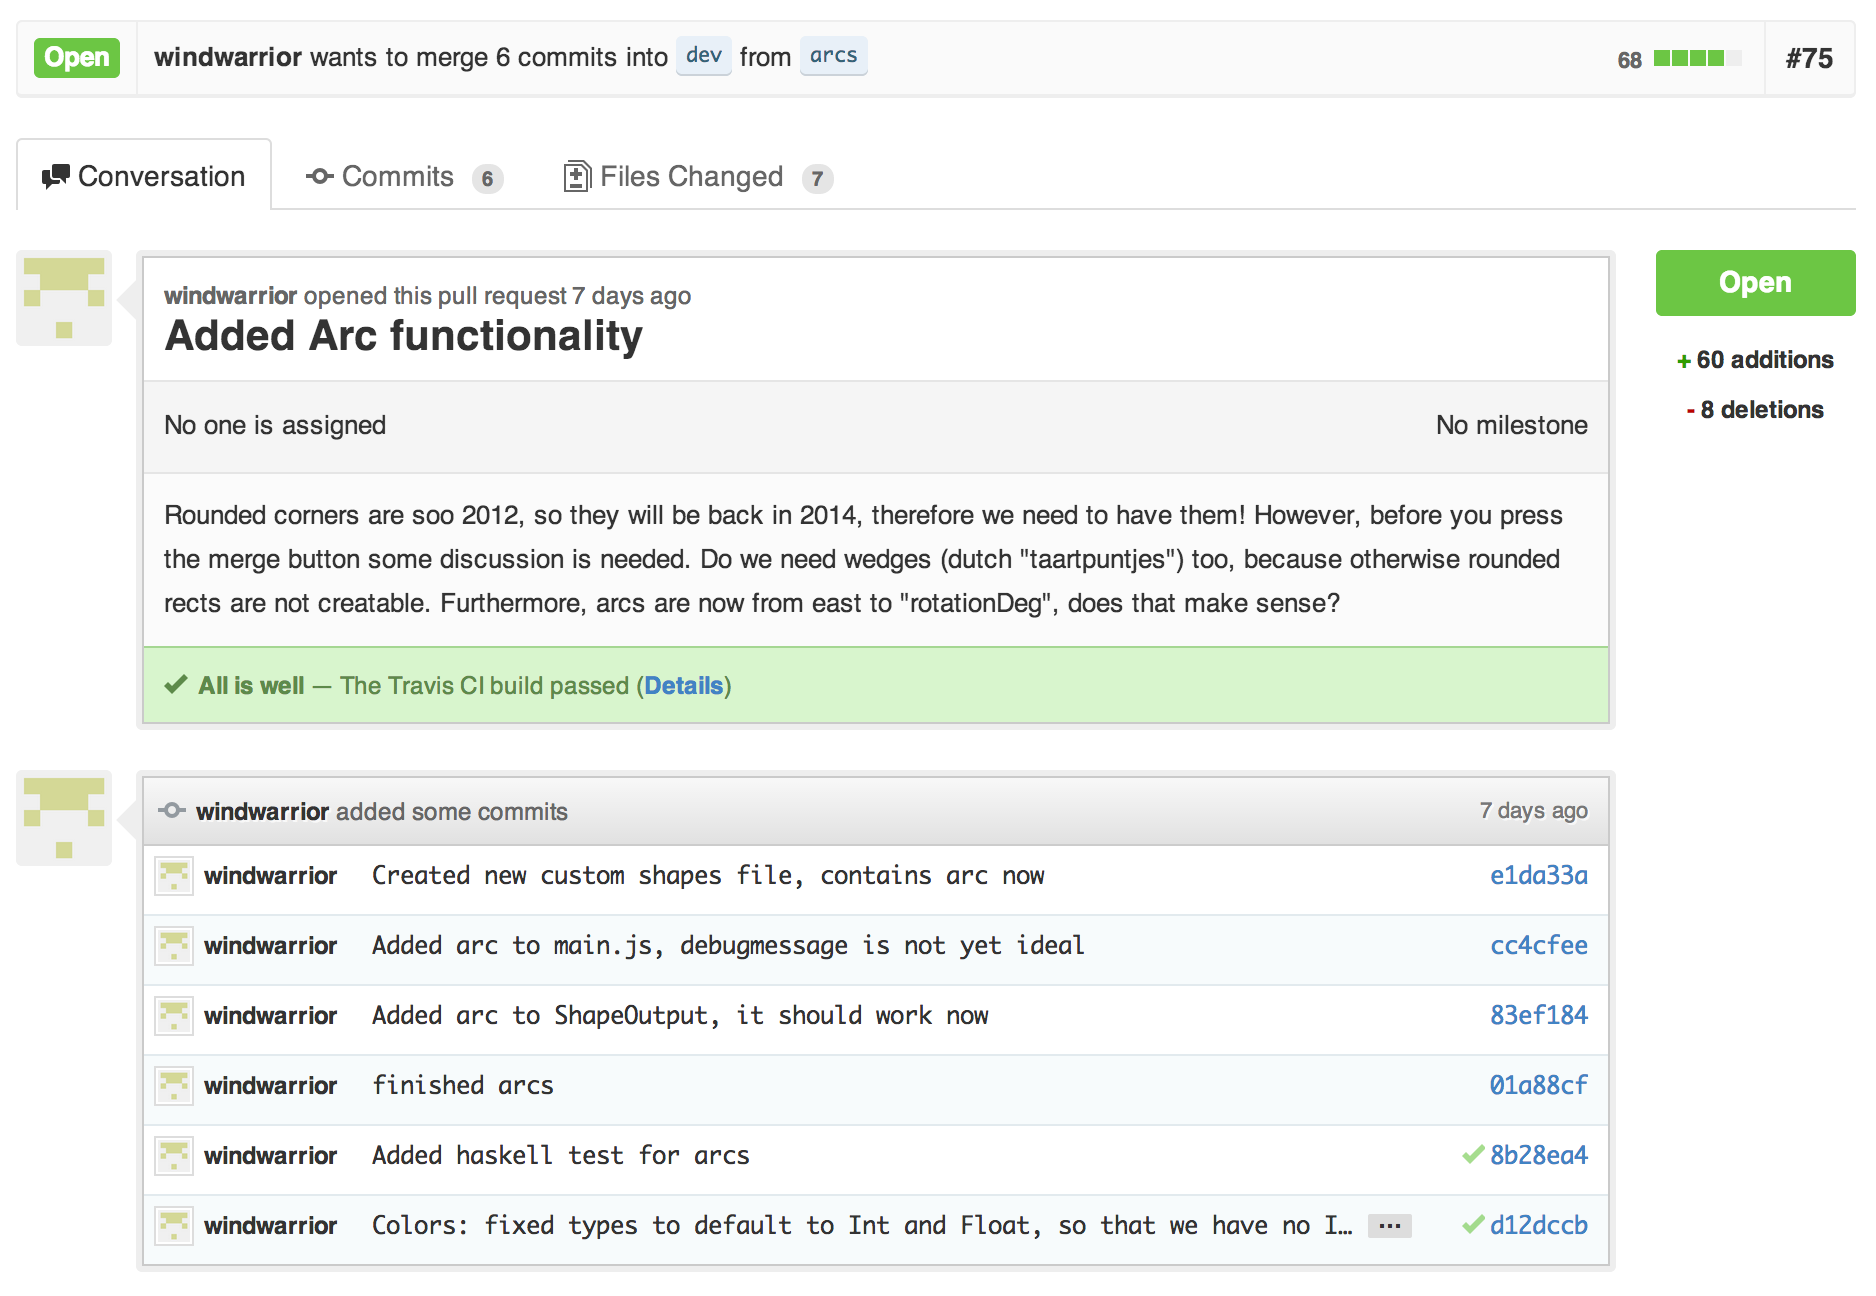
\includegraphics[keepaspectratio,width=\textwidth]{./images/pullrequest.png}
\caption{Pull Request \#75 Arcs geimplementeerd. – \url{https://github.com/CanvasHS/Canvas.hs/pull/75}}
\label{fig:pullrequest}
\end{center}
\end{figure}

Als een feature af is moet deze beoordeeld voordat deze gemergd kan worden naar de \inlinecode{dev} branch. Daarvoor wordt een \emph{pull request} aangemaakt. Deze \emph{pull request} bevat dan informatie over de wijzigingen tenopzichte van de versie die op de \inlinecode{dev} branch staat. Een beoordelaar kan de code lezen en deze goedkeuren. Op het moment dat de code goed wordt gekeurt komt een nieuwe versie met de nieuwe feature op de \inlinecode{dev} branch te staan.

Bij aanvang van het project was deze werkwijze voor veel teamleden nieuw. En daarom is het in het begin niet altijd juist toegepast. Maar naarmate het project vorderde is steeds vaker met succes gebruik gemaakt van het pull request principe. Dit zorgde er voor dat teamleden elkaars code controleerde en dat er minder bugs zaten in de versies op de \inlinecode{dev} branch.

\subsection{Continuous integration met Travis CI}

Om het beoordelen van code gemakkelijk te maken voor de ontwikkelaar en de beoordelaar is er gebruik gemaakt van de \emph{continuous integration} software \emph{Travis}. Deze software luistert naar nieuwe commits naar het centrale repository, als er een nieuwe commit gedaan is wordt er een virtuele machine opgestart die vervolgens middels een buildscript de versie van de software probeert te bouwen. Dit buildscript staat in de root directory van het repository.

Dit buildscript specificeert onder andere dat de software gebouwd moet worden met de Haskell compiler, maar ook dat alle geschreven tests uitgevoerd moeten worden. Mocht de compilatie of het uitvoeren van een van de tests niet geslaagd zijn is de build gefaald. Dit wordt dan vervolgens ook weergeven in het venster van de pull request. Als een beoordelaar ziet dat de build uit een pull request succesvol is, zoals bijvoorbeeld te zien bij \autoref{fig:pullrequest}, weet hij zeker dat de versie veilig is om te mergen.

Het buildscript voert naast de compilatie en de testen nog een paar andere commando's uit. Zo genereert het buildscript ook de documentatie en uploadet deze naar de Canvas.HS website—\url{http://canvashs.github.io}. Op de website kan de documentatie bekeken worden per build. Hierdoor hoeven ontwikkelaars zelf geen documentatie meer te genereren en hebben zij altijd, up to date, doorzoekbare documentatie.





 
\chapter{Requirements} \label{hoofdstuk:requirements}
Canvas.hs dient te voldoen aan verschillende requirements. Initieel is een lijst met requirements opgesteld; die deels zijn voortgekomen uit functionaliteit van de oude, op Gloss gebaseerde, grafische omgeving. Gedurende het ontwikkelproces zijn onder meer op basis van feedback van de opdrachtgever nieuwe requirements aan de orde gekomen. In dit hoofdstuk worden zowel oorspronkelijke als toegevoegde requirements opgenoemd en toegelicht.

In het kort dient de library te bestaan uit een browseromgeving die door middel van HTML en JavaScript een gebruikersinterface toont. Op deze gebruikersinterface moeten verschillende standaard figuren te tekenen zijn. En met de gebruikersinterface dient geinteracteerd te kunnen worden middels standaard invoer als toetsenbord en muis. Via een verbinding tussen de browseromgeving en de library kan er vanuit een Haskell-programma output gegenereerd worden in de browser en kunnen er events verstuurd worden vanuit de browseromgeving naar een Haskell-programma. Het deel van de library dat de verbinding met de browseromgeving opzet en onderhoudt wordt vanaf nu de \emph{module} genoemd. De module zal volledig geschreven zijn in Haskell.

De requirements zijn opgesteld met de MoSCoW-methode. Bij deze methode kunnen essenti\"ele, niet-essenti\"ele en uitgesloten requirements vastgesteld worden. Aan het eind van het project kan dan beter beoordeeld worden of alle essenti\"ele functionaliteit ge\"implementeerd is. Er wordt gebruik gemaakt van ``dient'' voor essenti\"ele requirements, ``kan eventueel'' voor niet-essentiele requirements en ``zal niet'' voor uitgesloten requirements. In de traceability matrix in \autoref{sec:traceability} wordt het eindproduct beoordeeld op basis van de requirements.

\subsubsection{Functionele requirements}
In de basis zal Canvas.hs dezelfde functionaliteit ondersteunen als de oude grafische omgeving die gebruik maakt van de Gloss library. De programmeur zou met deze library minstens even veel moeten kunnen weergeven. Om extra mogelijkheden te bieden dient de library ook animaties mogelijk te maken.

\newcounter{startvalue}
\begin{enumerate}[label={R\arabic*}]
	\item \label{req:prim} De library dient grafische primitieven zoals cirkels, rechthoeken, lijnen, Bézier curves, n-hoeken en tekst moeten op een simpele manier getekend kunnen worden vanuit het Haskell-programma van de student.
	\begin{enumerate}[label={R\arabic{enumi}.\arabic*}]
		\item \label{req:circle} De library dient cirkels te kunnen tekenen.
		\item \label{req:rect} De library dient rechthoeken te kunnen tekenen.
		\item \label{req:lines} De library dient lijnen te kunnen tekenen.
		\item \label{req:bezier} De library dient Bézier curves te kunnen tekenen.
		\item \label{req:text} De library dient tekst te kunnen tekenen.
		\begin{enumerate}[label={R\arabic{enumi}.\arabic{enumii}.\arabic*}]
			\item De library dient verschillende fonts te ondersteunen.
			\item De library dient bold en italic tekst te ondersteunen.
			\item De library dient verschillende font sizes te ondersteunen.
		\end{enumerate}
		\item \label{req:pictures} De library kan eventueel plaatjes inladen op het canvas.
	\end{enumerate}
	\item De library dient vul- en lijnkleuren van grafische componenten instelbaar te maken.
	\begin{enumerate}[label={R\arabic{enumi}.\arabic*}]
		\item \label{req:colors:lines} De library dient lijnkleuren instelbaar te maken.
		\item \label{req:colors:fill} De library dient vulkleuren instelbaar te maken.
		\item \label{req:colors:fill:gradient} De library kan eventueel gradients als vulkleur gebruiken.
	\end{enumerate}
	\item De library dient events vanuit JavaScript door te geven aan het Haskell-programma van de student.
	\begin{enumerate}[label={R\arabic{enumi}.\arabic*}]
		\item \label{req:event:key} De library dient toetsaanslagen vanuit de browser door te geven.
		\item \label{req:event:mouse} De library dient muisklikken vanuit de browser door te geven.
		\item \label{req:event:scroll} De library dient scroll-events vanuit de browser door te geven.
	\end{enumerate}
	\item Een programmeur moet grafische componenten aan kunnen passen zonder zijn programma te hoeven hercompileren.
	\begin{enumerate}[label={R\arabic{enumi}.\arabic*}]
		\item \label{req:action:animate} De library kan eventueel stapsgewijze aanpassingen geanimeerd weergeven.
		\item \label{req:zoom} De library kan eventueel zoomen en geschoven worden op de canvas.
	\end{enumerate}
	\setcounter{startvalue}{\value{enumi}}
\end{enumerate}

\paragraph{Acties} In de oude grafische omgeving worden een aantal \emph{acties} ondersteund die buiten de grafische output om werken. Acties worden gedefineerd als: vanuit de \emph{module} aangeroepen gebeurtenissen. Deze acties bieden complexe functionaliteit versimpeld aan de gebruiker aan. Hierbij kan gedacht worden aan: het openen van een tekstinvoerpop-up en de mogelijkheid om bestanden te verwerken. Door het gebruik van acties hoeft de gebruiker zelf geen I/O te gebruiken in zijn Haskell programma. Dit verlaagt het instapniveau om aan de gang te gaan met Haskell en een grafische omgeving. Om Canvas.hs breder inzetbaar te maken dient het als extra functionaliteit ook fullscreen weergegeven te kunnen worden. Dit is bijvoorbeeld handig in een presentatie.

\begin{enumerate}[label={R\arabic*}]
\setcounter{enumi}{\value{startvalue}}
	\item De library kan acties ondersteunen die in de client of door de module worden uitgevoerd.
	\begin{enumerate}[label={R\arabic{enumi}.\arabic*}]
		\item \label{req:action:prompt} De library kan eventueel tekstinvoer vragen met een pop-up.
		\item \label{req:action:fullscreen} De library kan eventueel fullscreen getoond worden.
		\item \label{req:action:localfiles} De library dient lokale bestanden te kunnen verwerken.
		\begin{enumerate}[label={R\arabic{enumi}.\arabic{enumii}.\arabic*}]
			\item De library dient lokale bestanden te kunnen openen via een functie die aangeboden wordt in de Haskell-module.
			\item De library dient lokale bestanden te kunnen wijzigen via een functie die aangeboden wordt in de Haskell-module.
		\end{enumerate}
		
		\item \label{req:action:userfiles} De library kan eventueel bestanden die de gebruiker aanbied verwerken.
	\end{enumerate}
	\setcounter{startvalue}{\value{enumi}}
\end{enumerate}

\paragraph{Gebruiksvriendelijkheid} Een van de voornaamste problemen met de oude grafische omgeving is de gebruiksvriendelijkheid van de library. Wanneer er een fout in het programma zat werd het direct afgesloten zonder daarbij een foutmelding te geven. Dit maakt het lastig om fouten in de programmatuur te vinden. Canvas.hs heeft daarom als doelstelling om een gebruiksvriendelijke omgeving aan te bieden die de programmeur duidelijke foutmeldingen geeft.

\begin{enumerate}[label={R\arabic*}]
\setcounter{enumi}{\value{startvalue}}
	\item \label{req:errors} De library dient duidelijke errors te genereren.
	\begin{enumerate}[label={R\arabic{enumi}.\arabic*}]
		\item Als de verbinding tussen JavaScript en Haskell verbroken wordt dient de library een error te tonen aan de gebruiker. 
		\item De library dient een error te tonen wanneer een functionaliteit in een onverwachte staat komt.
	\end{enumerate}
	\item \label{req:launchbrowser} De library dient automatisch een browser te starten bij het draaien van het programma.
	\item \label{req:reload} De library dient de browseromgeving opnieuw te laden als het Haskell-programma opnieuw gecompileerd wordt.
	\item \label{req:debug} De JavaScript-omgeving dient een simpele debug-console te bevatten.
	\setcounter{startvalue}{\value{enumi}}
\end{enumerate}

\subsubsection{Niet functionele requirements}
Operating systemen incompatibility was een ander probleem met de oude grafische omgeving. Hier moet Canvas.hs verandering in gaan brengen. Door gebruik te maken van HTML standaarden zal de library een goede basis hebben om platform onafhankelijk te werken. Om er voor te zorgen dat de library goed werkt en te onderhouden blijft dient het te voldoen aan een aantal kwaliteitseisen.

\begin{enumerate}[label={R\arabic*}]
\setcounter{enumi}{\value{startvalue}}
	\item \label{req:multiplatform} De library dient multiplatform te werken.
	\begin{enumerate}[label={R\arabic{enumi}.\arabic*}]
		\item De library dient te werken in de laatste versie van Internet Explorer, Firefox, Chrome en Safari.
		\item De library dient te werken op Linux, OS X en Windows.
		\item De library dient te werken op een computer met een hoge pixeldichtheid.
	\end{enumerate}
	\item \label{req:performance} De library dient gemakkelijk en snel te gebruiken te zijn.
	\begin{enumerate}[label={R\arabic{enumi}.\arabic*}]
		\item De library dient eenvoudig te installeren zijn.
		\item De library dient makkelijk af te sluiten te zijn.
	\end{enumerate}
	\item \label{req:maintenance} De library dient makkelijk te onderhouden zijn.
	\begin{enumerate}[label={R\arabic{enumi}.\arabic*}]
		\item De library dient gedocumenteert te zijn.
		\item De library dient modulair opgebouwd te zijn.
	\end{enumerate}
	\item \label{req:coverage} De library dient getest te zijn met 70\% code coverage (exclusief frameworks).
\end{enumerate} 
\chapter{Ontwerp} \label{hoofdstuk:ontwerp}

\section{Globaal ontwerp}  \label{sec:globaal}
Canvas.hs is een library die de programmeur kan importeren in zijn programma om er daarna met de API die Canvas.hs aanbiedt gemakkelijk een uitgebreide user interface mee te bouwen. Canvas.hs focust zich op elementaire input en geen ondersteuning heeft voor high level interface elementen zoals knoppen en textgebeiden. Deze elementen zijn met behulp van Canvas.hs gemakklijk te implementeren. \autoref{fig:demo_screenshot} geeft een demoapplicatie van Canvas.hs weer.

\todo{hier uitwijden over principe van Canvas.hs? Als het goed is al in inleiding gebeurd. Moet iig verteld zijn over hoe we een weegave hebben in een webbrowser met canvas, en een tussenliggende module die dat 'niet monadisch' mogelijk maakt}


\begin{figure}[H]
\begin{center}
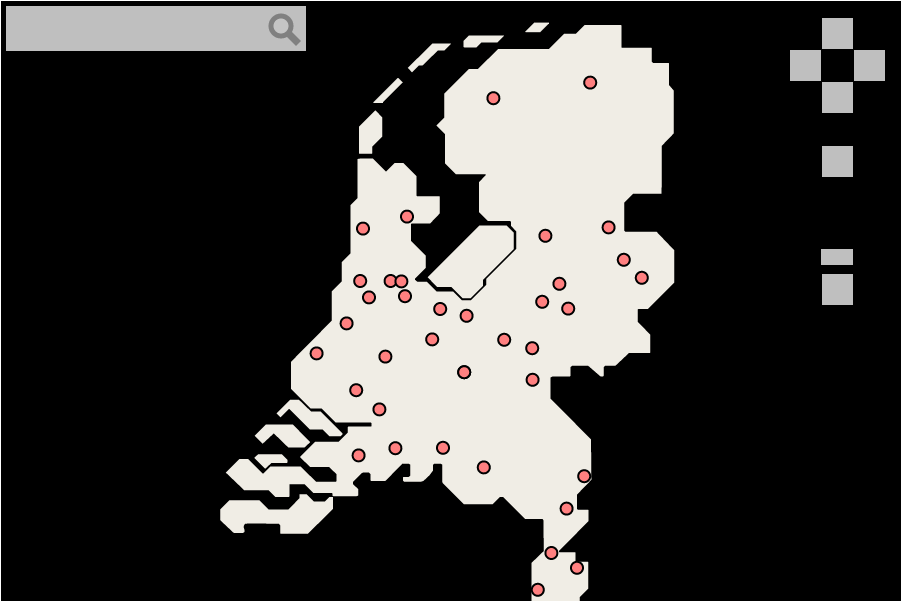
\includegraphics[keepaspectratio,width=\textwidth]{./images/demo.png}
\caption{Een demoapplicatie van de Canvas.hs library}
\label{fig:demo_screenshot}
\end{center}
\end{figure}


\autoref{fig:overzicht_architectuur} geeft een overzicht van de architectuur. Canvas.hs bestaat uit een module en een client. De module is een library die de programmeur in zijn programma importeert. Bij het starten van de module start een HttpServer, een WebSocket-server en wordt de webpagina van de client automatisch gestart. De client bestaat uit een browserpagina met onder andere een canvas element. De module communiceert met de client via een WebSocket verbinding om grafische elementen op de canvas in de client te tekenen.

\begin{figure}[H]
\begin{center}
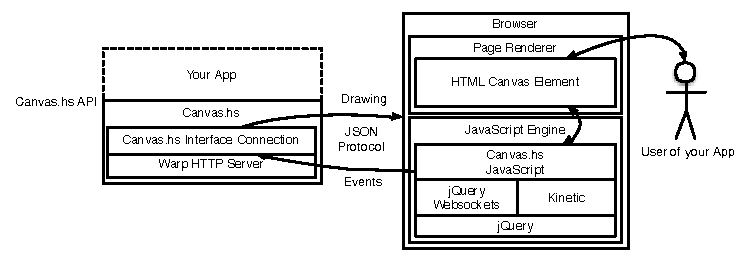
\includegraphics[keepaspectratio,width=\textwidth]{./images/architectuur_overzicht.pdf}
\caption{Overzicht van de architectuur van Canvas.hs}
\label{fig:overzicht_architectuur}
\end{center}
\end{figure}


Voor elke gebeurtenis (event, zoals bijvoorbeeld een muisklik) die binnen het systeem plaatsvindt wordt de code van de user applicatie aangeroepen. Deze eventHandler kan op basis van deze gebeurtenis een nieuwe grafische boom opleveren, hierbij kan gedacht worden aan een boom met daarin o.a. text en simpele vormen die samen een groter geheel vormen. Deze boom zal vervolgens op het canvas getekend worden. De eventhandler kan daarnaast ook nog een aantal uit te voeren acties opleveren, hierbij kan gedacht worden aan bijvoorbeeld het lezen of schrijven van bestanden. Daarnaast heeft de eventHandler de mogelijkheid om state bij te houden. Elke keer dat deze door Canvas.hs wordt aangeroepen krijgt deze de vorige opgeleverde state mee en de eventhandler heeft een nieuwe state in het resultaat. Het type van de eventHandler ligt dit duidelijk toe: \inlinecode{eventHandler :: a -> Event -> (a, Output)}, hierin is \inlinecode{a} de state die de eventHandler kan bijhouden. 


\autoref{eventHandler_voorbeeld_simpel} illustreeert een simpele eventHandler die bij de start van het programma (\inlinecode{StartEvent}) een vierkant tekent en een timer start. Vervolgens wordt elke keer dat deze Timer afgaat het vierkant verplaatst. Als state wordt een simpele \inlinecode{Int} gebruikt. D.m.v de installEventHandler functie van Canvas.hs wordt de eventHandler geregistreerd en het systeem gestart.

\begin{lstlisting}[caption=Voorbeeld van een simpele eventHandler, label=eventHandler_voorbeeld_simpel]
import CanvasHs
import CanvasHs.Data

type State = Int

main = installEventHandler handle 0

handle :: State -> Event -> (State, Output)
handle StartEvent st 	= (st+1, output)
	where 
		output = Out (shape, actions)
		shape = rectangle st
		actions = [Timer 1000 "move"]
		
handle (Tick "move") st	= (st+1, shape $ rectangle st)
		
rectangle :: Int -> Shape
rectangle i = Rect (10*i, 10*i) 10 10
\end{lstlisting}

Een gedetailleerde handleiding over Events, Shapes, Actions in het algemeen het gebruik van Canvas.hs kan gevonden worden in appendix A: gebruikerhandleiding. \todo{Invoegen referentie}

\paragraph{Shapes}
Zoals hierboven aangegeven levert de eventHandler o.a. een grafische boom op. Deze boom is gebasseerd op het Shapetype. Dit type definieert een aantal primitieven, zoals lijnen en vierkanten, en aantal translaties zoals verschuivingen en translaties die op een primitieve worden toegepast. Daarnaast wordt via het Shapetype ook aangegeven of er interesse is in events, zoals muiklikken, die plaatsheben op de Shape. In fig is een grafische boom van Shapes weergegeven. 

\todo{blablabla bilbiotheken gebriken om makkelijker te maken enzo}

\todo{detailontwerp doorlezen om te checken of nog andere dingen gemist zijn bij globaal ontwerp}

\section{Detail ontwerp} \label{sec:detail}

In deze sectie wordt uitgebreid ingegaan op het ontwerp van de library. Eerst wordt de architectuur toegelicht in \autoref{subsec:architectuur} waar onder andere ingegaan wordt op de communicatie tussen de \emph{module} en de \emph{client}.

In \autoref{subsec:externe_libraries} wordt uiteengezet wat welke overwegingen hebben geleid tot het gebruik van verschillende extrerne libraries/dependencies. Daarna wordt dieper ingegaan op de werking can de \emph{module}, de \emph{client} en ondervonden problemen. Tot slot wordt de het ontwerp voor de werking van de grafische bibliotheek verder toegelicht in \autoref{subsec:grafische_bibliotheek}.

\subsection{Architectuur}
\label{subsec:architectuur}

De applicatiearchitectuur die Canvas.hs gebruikt bestaat uit drie componenten. De applicatie van de gebruiker, de Canvas.hs module en de JavaScript Canvas.hs applicatie—in dit verslag aangeduid als de client. De module en de client vormen samen de Canvas.hs library.

De Canvas.hs module biedt functies aan die de programmeur kan gebruiken om te tekenen en bepaalde acties uit te voeren in de browser. De module draait een server om te communiceren met de client. De client verbindt door middel van websockets met de server en geeft de output van het programma weer in een canvas HTML-element. In \autoref{fig:architectuur} is een schematische weergave van de architectuur weergegeven.

\begin{figure}
\begin{center}
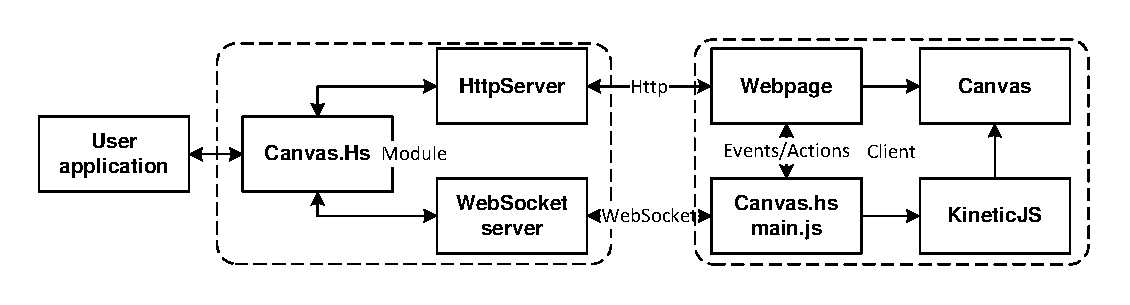
\includegraphics[keepaspectratio,width=\textwidth]{./images/architecture.pdf}
\caption{Architectuur van Canvas.hs}
\label{fig:architectuur}
\end{center}
\end{figure}

\subsubsection{Communicatie}
Gegevensoverdracht tussen de HTTP server en de browser moet snel gebeuren. Om de grafische elementen in de browser weer te geven moeten de output van de grafische interface naar de browser gecommuniceerd worden. Wanneer de gebruiker interactie heeft met de interface moet dit naar het programma van de gebruiker gecommuniceerd worden. Verder zal het programma bepaalde acties moeten kunnen uitvoeren op de webbrowser, zoals fullscreen laten gaan van de browser. Een belangrijke overwegingen is dat de grafische interface zo min mogelijk vertraging moet hebben.


\paragraph{Websockets}
Het is mogelijk om door middel van XMLHttpRequest of WebSockets een verbinding te onderhouden tussen de Module en de Clientomgeving. XMLHttpRequests worden door alle webbrowsers ondersteund, en kan door middel van longpolling technieken (Comet) \todo{PJ: wat is deze? of meer uitleg of verwijzingkje denk ik} een verbinding onderhouden met de webserver. De meest recente browsers ondersteunen WebSockets. Dit biedt een socket verbinding tussen de client en de server. Het WebSockets protocol biedt een betere performance dan alle technieken op basis van XMLHttpRequests en biedt een groter implementatiegemak. Door het gebruik van het HTML canvaselement zal de browser ondersteuning al beperkt zijn tot de meest recente browsers. Canvas.hs maakt gebruik van WebSockets.

\paragraph{Protocol}
In Cavas.hs wordt voor deze communicatie gebruik gemaakt van JSON \cite{JSON2006}. JSON staat voor JavaScript Object Notation en is een notatie waarin objecten als text worden gerepresenteerd zoals dit ook in Javascript wordt gedaan. JSON is een veel gebruikte notatie voor communicatie met Javascript. Het voordeel van JSON is, doordat het zo veel gebruikt wordt, dat er veel bibliotheken beschikbaar zijn om met JSON om te gaan. Zowel voor javascript als voor Haskell was het eenvoudig een goede externe bibliotheek te vinden om data van en naar JSON te lezen en te schrijven. Een ander groot voordeel van JSON is dat het, in tegenstelling tot bijvoorbeeld XML, weinig overhead heeft. Een uitgebreide handleiding van het protocol van gevonden worden in \cite{Protocol2013}.

Het protocol tussen de client en de server bevat voornamelijk interface data. De structuur en de attributen moeten vertaald worden van de Haskell omgeving om gebruikt te worden om te tekenen in het Canvas en vervolgens input van de gebruiker in de client te ondersteunen. De datastructuur van het protocol lijkt zoveel mogelijk op die van het canvas. Hierdoor kan data die binnenkomt bij de javascript applicatie zonder al te veel veranderingen op het canvas getekend worden.

\paragraph{Stateless module}
De Canvas.hs module houdt de huidige grafische boom niet bij. Deze wordt na ontvangst van de gebruiker applicatie onmiddelijk geëncodeerd naar JSON en opgestuurd naar de Javascriptapplicatie. Dit heeft een aantal voordelen, allereerst maakt dit het gebruik van de module door de programmeur gemakkelijker. Elke keer dat de eventHandler wordt uitgevoerd wordt hiervan verwacht dat deze een volledige grafische boom oplevert. Hierdoor is het voor de programmeur en de module niet nodig om uit te zoeken waar de grafische boom precies veranderd moet worden. Bijkomend voordeel hiervan is dat er slechts één plek is waar de huidige grafische boom wordt bijgehouden: de Javascript applicatie. Hierdoor kunnen er geen synchronisatiefouten tussen de Haskell module en de Javascriptapplicatie ontstaan. 

Nadeel van deze aanpak is dat er veel overhead is door het voortdurend versturen van de volledige grafische boom. Zelfs voor het verplaatsen van één object moet de hele boom opnieuw verstuurd worden. Dat er veel data verstuurd wordt levert geen problemen op doordat het systeem ontwikkeld is voor lokaal gebruik en data over websockets lokaal zeer snel verstuurd wordt. De aanpak levert wel problemen op als er snel veel getekend wordt, doordat het tekenen naar het canvas in onze aanpak relatief veel tijd kost. Hier wordt verder op gereflecteerd onder conclusie.\todo{Dit daadwerkelijk doen, referentie invoegen}
\subsection{Externe libraries}

\subsubsection{Webserver}
Om de statische files van onze library te serveren hebben we een HTTP-server nodig, we hebben hier gekozen voor ``warp''. Warp bied een lichtgewicht webserver die goed gedocumenteerd en ondersteund is. Andere opties waren ``happstack'', ``hyena'' en ``snap server"". Dit zijn eigenlijk volledige webframeworks, wij hoefden slechts statische files te serveren. Voor de eenvoud en onderhoudbaarheid was ``warp'' de beste keuze.

\subsubsection{Websocketserver}
De websocketserver is degene die connecties tussen de Haskell en Javascript onderhoud, we hebben hier gekozen voor de ``websockets'' library. Er had gekozen kunnen worden om hieromheen de ``wai'' wrapper te gebruiken, maar omdat we weinig gebruik maken van andere functionaliteit van ``wai'' hebben we het bij de normale library gehouden.

Binnen de websockets zijn er verschillende protocollen gedefineerd, welke in verschillende browsers geimplementeerd zijn. De meest recente versie van het websockets protocol poogt een standaard te worden (RFC6455) en de websockets library heeft daar tijdens ons ontwerpproject support voor gekregen. De meeste recente browsers hebben RFC-6455 geimplementeerd, en de verwachting is dat deze versie van het protocol lange tijd ondersteund wordt.

\subsubsection{JSON}
Binnen ons protocol gebruiken we JSON. In eerste instantie wilden we hiervoor een eigen parser schrijven, we waren namelijk sceptisch over het gebruik van een library omdat het parsen van JSON niet moeilijk lijkt terwijl de libraries ingewikkeld leken. Uiteindelijk hebben we toch een library genomen, libraries vertrouwde stukken code zijn waarvan al geverifieerd is dat ze werken, daartoe bespaart het ons veel tijd en hebben we een solide basis van onze code.

Er zijn voor haskell twee bekende JSON libraries, Text.JSON en Aeson. In eerste instantie hebben we gekeken naar Text.JSON maar al snel bleek dat deze library slecht gedocumenteerd is. Daarna hebben we naar Aeson gekeken, Aeson is beter gedocumenteerd en bied eenzelfde workflow.
Binnen Aeson is er gekozen om Template Haskell functies te gebruiken, dit is een GHC extensie die een soort van metaprogramming toevoegd aan Haskell. Template Haskell is gebruikt om lege keys uit de JSON te verwijderen en een record probleem van Haskell te omzeilen.

\subsubsection{Tests}
Als testingframework hebben we voor Hspec gekozen. Hspec intergreerd goed met andere testframeworks zoals QuickCheck en HUnit maar daarbovenop voegt het verhalende syntax toe aan de testcases. Ook zoekt Hspec automatisch naar testcases, en paralleliseerd het testcode.

Binnen Hspec maken we ook gebruik van QuickCheck, deze library kan arbitraire testcases testen. Hiervoor dient de input gedefineerd te worden en dan zal QuickCheck een groot aantal testcases loslaten op de code. Vaak gebruiken we eerst een voorgedefineerde testcase (van HSpec zelf, wat weer een wrapper om HUnit is), en daarnaast een arbitrair aantal extra testcases gegenereerd door QuickCheck. Zo weten we dat het geen toeval was dat onze tests checkte en kunnen we zonder al te veel moeite veel gevallen proberen.

\subsection{Module}
De module is de Haskell bibliotheek die de programmeur gebruikt om de grafische interface in de client te bedienen. Naar de programmeur is de gebruiksvriendelijkheid van de biblotheek een van de belangrijkste overwegingen voor het ontwerp. De module bestaat uit een aantal onderdelen: de server die de statische bestanden serveert, de websocket server die de verbinding met de client onderhoud, en de laag die de input en output verwerkt. \autoref{fig:architecture_module} geeft de architectuur weer van de module.

\begin{figure}
\begin{center}
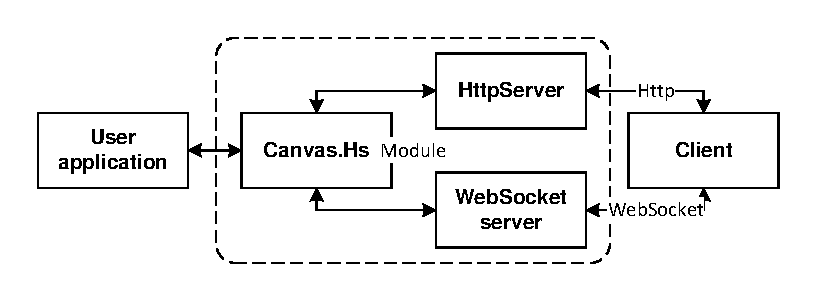
\includegraphics[keepaspectratio,width=\textwidth]{./images/module_architecture.pdf}
\caption{Architectuur van de module}
\label{fig:architecture_module}
\end{center}
\end{figure}

\paragraph{Servers}
Canvas.hs draait een simpele server op port 80 die statische bestanden kan serveren. Waaronder de index pagina, de javascript bestanden en eventueel plaatjes. Op port 8080 draait een websocket server die de verbinding met de client onderhoud.


\paragraph{Server in de module}
De server draait in het process wat gestart wordt vanuit de Haskell-code van de programmeur. De main van de programmeur start (indirect) de server. Dit is envoudiger dan het draaien van de server in een apart process. Er hoeft namelijk niet tussen verschillende Haskell-processen gecommuniceerd te worden. Dit scheelt het schrijven van nog een interface tussen het server- en het module process. Nadeel is wel dat het voortdurend opnieuw starten en afsluiten van de server leidt tot vertraging in het opstarten van het programma van de programmeur. Dit is vervelend als de programmeur regelmatig kleine wijzigingen maakt en dan de code opnieuw moet starten. Echter lijkt de overhead van het opnieuw starten van de server minimaal. Het is verder praktisch dat er geen rekening gehouden hoeft te worden met de state van de server bij het opstarten van het programma.

\paragraph{Gebruik} Wanneer de programmeur gebruik wil maken van de Canvas.hs moet hij gebruik maken van de installEventHandler functie. Bij het aanroepen van deze functie moet de programmeur een event handler meegeven die alle events vanuit de interface afhandeld. Om het gebruik van Canvas.hs zo makkelijk mogelijk te houden zal bij het aanroepen van installEventHandler automatisch de statische server en de websocket server gestart worden, en daarna automatisch de browserpagina geopend worden. \autoref{fig:startup_procedure} geeft de opstartprocedure weer.

\begin{figure}
\begin{center}
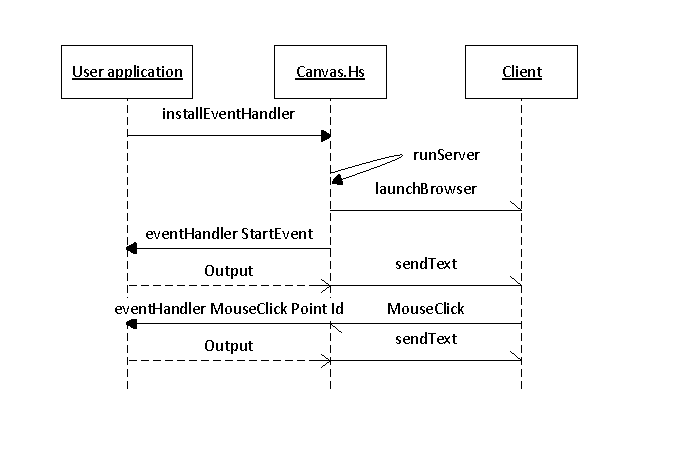
\includegraphics[keepaspectratio,width=\textwidth]{./images/module_startup_procedure_interaction.pdf}
\caption{De opstartprocedure en initiele interactiesequentie}
\label{fig:startup_procedure}
\end{center}
\end{figure}

\paragraph{Input/output}
De module handeld input en output af door events naar de eventhandler van de programmeur te sturen. Bijvoorbeeld: wanneer een gebruiker op een rondje klikt zal het programma de event handler aanroepen met de ID van dat rondje en de lokatie van de muisklik. De event handler van de programmeur kan dan nieuwe output genereren op basis van dit event. Zoals een nieuw menu weergeven of het uitvoeren van een actie zoals het opvragen van een bestand van de gebruiker.In \autoref{fig:startup_procedure} is deze interactie weergegeven.

De programmeur zal in zijn eventhandler bij ieder event de huidige state en de huidige event meekrijgen. Het type van de eventhandler is \inlinecode{userState -> Event -> (userState, Output)}, waarin de programmeur elk type aan userState kan geven. Door middel van pattern matching kan de programmeur makkelijk een bepaald event opvangen. Een muisklik event wordt opgevangen door: \inlinecode{handler state (MouseClick (x,y) "id")}. De returnwaarde vand de eventhandler is een tuple van de nieuwe state en de output. Output is een tuple van \inlinecode{(Maybe Shape, [Action])}. De eventhandler kan meerdere acties tegelijk uitvoeren en/of een grafische output leveren. De ondersteunde events en outputtypes worden verder toegelicht in \autoref{subsec:grafische_bibliotheek}.

-TODO: Acties   
\paragraph{Timers}
Canvas.Hs ondersteund timers die ervoor zorgen dat met een bepaald interval een event naar de eventhandler wordt verstuurd. Hiermee kunnen bijvoorbeeld animaties worden toegevoegd aan de interface. Deze timers worden bijgehouden in de module. Een alternatief is om de timers aan de client over te laten. Dit heeft als voordeel dat het makkelijker is om timers bij de houden in JavaScript dan in Haskell. In Haskell ontstaan er dan verschillende threads die je moet bijhouden. Groot voordeel is dat er geen extra acties over de WebSocketconnectie verzonden hoeven worden en dat een implementatie direct in Haskell meer precisie geeft voor de timer.

\paragraph{Unsafe I/O}
In Server.hs wordt gebruik gemaakt van unsafePreformIO voor het starten van child processen (een MVar die threads bijhoudt) en om een verbinding met een client bij te houden (een IORef die de connections naar de clients bevat). Hoewel het in dit geval volkomen veilig is, zijn er bezwaren tegen het gebruik van unsafePerformIO\cite{Haskell.org2008}. Dit is namelijk niet de netste oplossing en kan meestal voorkomen worden. Het is netter om een Server Monad te gebruiken die een State implementeert die deze zaken bijhoudt. Echter is het implementeren daarvan tijdsintensief, waardoor voor deze oplossing is gekozen.

\subsection{Client}
Het voornaamste onderdeel van de client is het canvas-element waarin de output getekend wordt door Kinetic.js. Daarboven zit de Canvas.hs javascriptcode die de verbinding onderhoud met de module en dit doorspeeld naar Kinetic.js om te tekenen. In dit deel worden voornamelijk de ontwerpbeslissingen besproken die betrekking hebben op de werking met KineticJS en de webbrowser.

\begin{figure}
\begin{center}
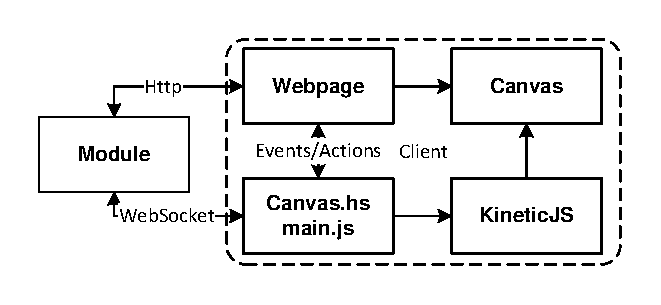
\includegraphics[keepaspectratio,width=\textwidth]{./images/client_architecture.pdf}
\caption{Architectuur van de JavaScript client}
\label{fig:architecture_client}
\end{center}
\end{figure}

\subsubsection{Canvas/Events}
Vanuit de module ontvangt de client via de WebSocket verbinding output. Ieder element wordt omgezet en aangemaakt in KineticJS. Voor elk element dat geinteresseerd is in een event wordt een eventlisteners toegevoegd. Wanneer de volledige structuur opgebouwd is wordt door oude structuur weggegooid en de nieuwe structuur op het canvas getekend.

\paragraph{Mousedrag}
Standaard ondersteund KineticJS mousedrag events, maar door de manier waarop Canvas.hs iedere keer opnieuw de output genereert raken de events van KineticJS verloren. Daarom maakt Canvas.hs gebruik van een eigen implementatie van mousedrag in de Canvas. Een mousedrag begint met een MouseDownEvent. Vanaf dat moment houd de client een ID bij van het huidige element. Alle opvolgende MouseMoveEvents zijn drag events die naar de client worden verstuurd. Deze MouseMoveEvents worden dooregegeven naar de Haskell kant met de vorige coördinaten van de muis en de huidige coördinaten van de muis.
Op deze manier kan de Haskell kant bepalen wat er moet gebeuren tijdens het draggen. Op het moment dat het programma aangeeft niet meer geinteresseerd te zijn in drag events op dat ID of in het geval van een MouseUpEvent stopt de drag in de client.

\subsubsection{Acties}
De programmeur kan een aantal specifieke acties uitvoeren op de client. De state van deze acties wordt onderhouden door de client zelf.
-TODO: Referentie naar de specifieke sectie in de grafische bibliotheek

\paragraph{Browserrestricties}
Canvas.hs bied de optie om de canvas in volledigscherm te laten weergeven. Door veiligheidsfunctionaliteiten in de huidige webbrowsers is het niet mogelijk om direct naar volledigscherm te gaan met behulp van JavaScript. Dit is alleen mogelijk vanuit klik- en toetsenbordevents. Daarom krijgt de gebruiker eerst een menu te zien voordat de browser naar volledigscherm gaat. Dezelfde veiligheidsrestricties zijn er voor het bestandenselectiemenu hierdoor heeft Canvas.hs daar ook een menu voor.

-TODO: Referentie naar de grafische bibliotheek over volledigscherm

\paragraph{Debug Console}
Voor de programmeur die gebruik gaat maken van de Canvas.hs library is het belangrijk dat zijn interface er zo uit ziet zoals hij dit wil. Ongetwijfeld zal een programmeur tegen problemen aanlopen bij het bouwen van de interface die hij niet had voorzien bij het schrijven van zijn code. Om probleemoplossing hiervan te vergemakkelijken bevat Canvas.hs een debug console bevat waar het aanroepen van teken functies en de invloed van deze API aanroepen goed visueel en tekstueel inzichtelijk worden. Doormiddel van een actie vanuit het programma van de gebruiker kan de debug console tevoorschijn gehaald worden.
\subsection{Grafische bibliotheek} \label{subsec:grafische_bibliotheek}

-TODO: Ontwerpkeuze: Referentie van specifieke elementen met behulp van ID toelichten
 
\chapter{Testplan} \label{hoofdstuk:testplan}
Gedurende het gehele ontwikkelingstraject zullen tussenreslultaten getest moeten worden. Het heeft de voorkeur dat dit vaak gebeurd zonder dat er veel tijd nodig is voor het uitvoeren van de tests. Voor elke requirement, feature en elk object moet een bijbehorende test worden ontwikkeld.

In het eerste deel van dit hoofdstuk zal voornamelijk beschreven staan hoe de automatische testen zijn opgezet. Doordat Canvas.hs gebruik maakt van verschillende programmeer talen zijn er uiteindelijk ook meerdere testtechnieken en libraries nodig om alles goed te testen en te meten. Maar omdat sommige requirements gemakkelijker automatisch te testen zijn dan andere zullen uiteindelijk ook een aantal requirements getest worden door een gebruiker in plaats van door een computer.

De geschreven tests kunnen gemakkelijk uitgevoerd worden via \emph{Cabal}, een gereedschap dat gebruikt wordt bij programmeren in Haskell. Deze geschreven tests testen zowel de Haskell code als de JavaScript code. De testconfiguraties voor beide typen tests worden in het Cabal-bestand bijgehouden. Met het commando \inlinecode{Cabal test} kunnen alle tests van het project uitgevoerd worden. Op de website van Canvas.hs staan uitgebreide instructies over het uitvoeren van tests. \url{http://canvashs.github.io/test.html}

\section{JavaScript} 
Aan de client side wordt gewerkt met JavaScript. Het Jasmine\cite{Jasmine} test framework wordt gebruikt om de tests hiervoor te ontwikkelen. Door middel van PhantomJS\cite{PhantomJS} kunnen de tests vanaf de command prompt worden uitgevoerd zonder browser. Hierdoor kunnen de tests ook op de build server uitgevoerd worden. Verder wordt er gebruik gemaakt van de imagediff\cite{imagediff} library om getekende output te testen. Voor het meten van code coverage in JavaScript wordt gebruik gemaakt van Blanket.js\cite{Blanket.js}.

\section{Haskell}
De Haskell-code in Canvas.hs wordt getest met behulp van \emph{Hspec}\cite{Hspec}. Hier is voor gekozen omdat Hspec relatief eenvoudig werkt en goed integreert met Cabal. Hierbij kan Hspec automatisch de verschillende tests in een bestandsmap ontdekken en uitvoeren.

In samenwerking met Hspec wordt \emph{QuickCheck}\cite{QuickCheck} gebruikt. Dit veel gebruikte testframework maakt het mogelijk om een groot aantal willekeurige testcases uit te voeren. Dit geeft extra zekerheid over de geteste code aangezien er naast de bekende edge cases, waarvoor tests in Hspec zijn geschreven, ook een groot aantal willekeurige cases wordt getest.

\section{Continuous Integration}
Zoals eerder genoemd in \autoref{sec:technische_organisatie} is er tijdens het project gebruik gemaakt van automatisch testen. Iedere ontwikkelaar stuurt gedurende de ontwikkeling zijn aanpassingen naar de centrale repository. Deze centrale repository is gekoppeld met Travis, een cloud-based continuous integration server. Travis voert automatisch tests uit na elke commit die naar de repository gestuurd is. Indien Travis fouten detecteert bij het draaien van de tests wordt dat aan de ontwikkelaars gemeld. Doordat de code automatisch getest wordt is altijd duidelijk welke bij welke commit fouten in worden introduceert, wat de status van iedere branch is en of een branch gemergd kan worden naar de development branch.

\section{Blackbox}
Naast de automatische tests voor verschillende functionele requirements zullen ook een aantal niet-functionele requirements getest moeten worden. Hiervoor is het lastig automatische testen te schrijven. Hierbij zal het vooral gaan om de cross-platform requirements beschreven in \autoref{hoofdstuk:requirements}. Hiervoor zullen verschillende demo applicaties in verschillende browsers en besturingssystemen getest worden.
 
\chapter{Resultaten} \label{hoofdstuk:resultaten}

\section{Testplan} \label{sec:testplan}
Gedurende het gehele ontwikkelingstraject moeten tests ontwikkeld worden. Voor elke requirement, feature en elk object moet een bijbehorende test worden ontwikkeld. Om voldoende test coverage te garanderen moet alle ontwikkelde code gecontroleerd zijn op het hebben van tests voordat het in de centrale development branch geplaatst mag worden. Dit gebeurt door middel van feature branches  Iedere feature wordt in een aparte branch ontwikkeld, voordat een feature gemerged mag worden naar de dev branch moet een pull request gemaakt worden op github. Deze pull request wordt dan beoordeeld door twee andere personen op code coverage, code netheid, documentatie en de requirements. Wanneer dit in orde is wordt de code gemerged naar de dev branch. Zie  \autoref{fig:branching} voor de branchingstrategie.

\begin{figure}
\begin{center}
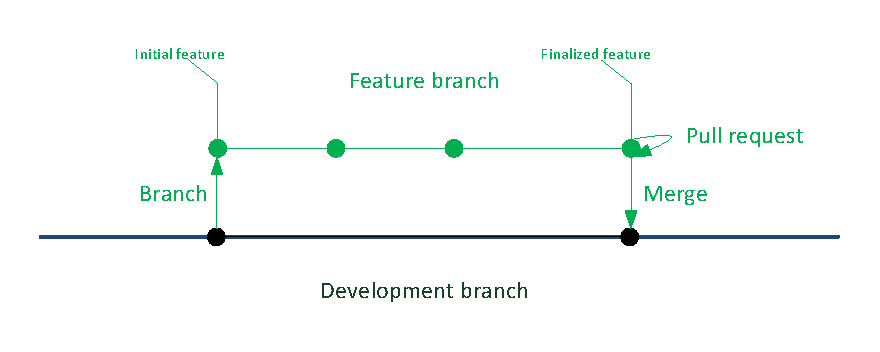
\includegraphics[keepaspectratio,width=\textwidth]{./images/branching.pdf}
\caption{Branching strategie van Canvas.hs}
\label{fig:branching}
\end{center}
\end{figure}

Door deze manier van werken is altijd de development branch goed getest en is het altijd mogelijk om een nieuwe release uit te brengen met de op dat moment volledig geteste features. Iedere release wordt in de master branch uitgebracht.

\subsection{Cabal}
De buildconfiguratie en testconfiguraties worden in de cabal file bijgehouden. Met het commando cabal test kunnen alle tests van het project uitgevoerd worden. Op de website van Canvas.hs staan uitgebreide instructies over het uitvoeren van tests.

\subsection{Continuous Integration}
Iedere ontwikkelaar zal gedurende de ontwikkeling zijn\todo{anders formuleren geen Engelse woorden er in dumpen} aanpassingen pushen naar de Github repository. De Github repository is gekoppeld met Travis een cloud based continuous integration server. Tests worden automatisch uitgevoerd door Travis na het pushen van iedere commit. Indien een build faalt, zal hierover een bericht in Hipchat geplaatst worden. Doordat builds automatisch getest worden is altijd duidelijk: Welke ontwikkelaar fouten in Canvas.hs introduceert, wat de status van iedere branch is en of een branch gemerged kan worden naar de development branch.

\todo{Beter alle losse delen geschrijven}
\todo{Duidelijkere TODOs schrijven want deze is mij compleet onduidelijk??}
\subsection{JavaScript} 
Aan de client side wordt gewerkt met JavaScript, het Jasmine test framework wordt gebruikt om de tests te ontwikkelen. Door middel van PhantomJS kunnen de tests vanaf de command line worden uitgevoerd zonder browser. Hierdoor kunnen de tests ook op de build server uitgevoerd worden. Verder zal er gebruik gemaakt worden van de imagediff library om de daadwerkelijk getekende output te testen. Voor het meten van code coverage in JavaScript wordt gebruik gemaakt van Blanket.js.

\subsection{Haskell}
De server en de module worden ontwikkeld met Haskell. Het Hspec test framework wordt gebruikt om deze onderdelen te testen. Voor het meten van de code coverage in Haskell wordt gebruik gemaakt hpc.

\section{Testresultaten} \label{sec:testresultaten}
Zoals in \autoref{hoofdstuk:testplan} beschreven zijn er verschillende tools en libraries gebruikt voor het automatisch testen van de functionele requirements. Daarnaast is er een aanpak voor het testen van de niet-functionele requirements. In dit hoofdstuk staan de resultaten van de tests voor zowel de functionele als niet-functionele requirements beschreven.

De resultaten van de automatische tests kunnen gecontroleerd worden door deze zelf uit te voeren. Een uitgebreide uitleg over het uitvoeren en ontwikkelen van tests is te vinden op de website van Canvas.hs: \url{http://canvashs.github.io/test.html}.

\subsection{JavaScript}
Voor de JavaScript-code zijn unit tests ontwikkeld in Jasmine. Met behulp van Blanket.js is de code coverage van de tests gemeten. Hieronder wordt de lijst met testcases weergegeven van de JavaScript-code. Alle test cases worden correct uitgevoerd.

\subsubsection{Testcases}
\newcounter{startvaluetest}
\begin{enumerate}[label={T\arabic*}]
	\item Execute actions
	\begin{enumerate}[label={T\arabic{enumi}.\arabic*}]
		\item \label{test:js:execute:actions:fixedsize} set fixed proportions
		\item \label{test:js:execute:actions:fluidsize} set fluid proportions
		\item \label{test:js:execute:actions:displayfixed} set window display type fixed
		\item \label{test:js:execute:actions:displayfluid} set window display type fluid
		\item \label{test:js:execute:actions:opencontrol} open control window
		\item \label{test:js:execute:actions:closecontrol} close control window
	\end{enumerate}
	\item Parse and run actions
	\begin{enumerate}[label={T\arabic{enumi}.\arabic*}]
		\item \label{test:js:parse:actions:no} parse no actions
		\item \label{test:js:parse:actions:fixedsize} parse fixedsize action
		\item \label{test:js:parse:actions:fluidsize} parse fluidsize action
		\item \label{test:js:parse:actions:fullscreen} parse fullscreen action
	\end{enumerate}
	\item Convert colors
	\begin{enumerate}[label={T\arabic{enumi}.\arabic*}]
		\item \label{test:js:convert:rgbajson:rgba} converts rgba json to rgba
		\item \label{test:js:convert:rgbajson:rgba:alphazero} converts rgba json to rgba with zero alpha
		\item \label{test:js:convert:rgbjson:rgba} converts rgb json to rgba
	\end{enumerate}
	\item Parse elements
	\begin{enumerate}[label={T\arabic{enumi}.\arabic*}]
		\item \label{test:js:parse:rect} parses a rectangle
		\item \label{test:js:parse:circle} parses a circle
		\item \label{test:js:parse:container} parses a container
	\end{enumerate}
	\item Draw elements
	\begin{enumerate}[label={T\arabic{enumi}.\arabic*}]
		\item \label{test:js:draw:line} draws a line
		\item \label{test:js:draw:rect} draws a rectangle
		\item \label{test:js:draw:polygon} draws a polygon
		\item \label{test:js:draw:arc} draws an arc
		\item \label{test:js:draw:circle} draws a circle (using rgb)
		\item \label{test:js:draw:circle:alpha} draws a circle with stroke alpha zero
		\item \label{test:js:draw:text} draws text
		\item \label{test:js:draw:container} draws container
		\item \label{test:js:draw:container:clipping} draws container with clipping
	\end{enumerate}

	\item \label{test:js:mouse} Mouse events
	\begin{enumerate}[label={T\arabic{enumi}.\arabic*}]
		\item \label{test:js:mouse:no} no event handlers
		\item \label{test:js:mouse:create} creating mouse event handlers
		\item \label{test:js:mouse:drag} creating mousedrag event handler (special case compared to other mouse event handlers)
	\end{enumerate}
	\item \label{test:js:mouse:draw} Draw elements to test event handling
	\begin{enumerate}[label={T\arabic{enumi}.\arabic*}]
		\item \label{test:js:draw:mousedown} message after mousedown event
		\item \label{test:js:draw:mouseclick} message after mouseclick event
		\item \label{test:js:draw:mouseup} message after mouseup event
		\item \label{test:js:draw:mousedoubleclick} message after mousedoubleclick event
		\item \label{test:js:draw:mouseover} message after mouseover event
		\item \label{test:js:draw:mouseout} message after mouseout event
		\item \label{test:js:draw:mousedrag} message after mousedrag event
		\item \label{test:js:draw:mousedragend} drag end after change of shape
		\item \label{test:js:draw:mousenodragend} no drag end after change of shape type
	\end{enumerate}
	\item Test realX and realY functions
	\begin{enumerate}[label={T\arabic{enumi}.\arabic*}]
		\item \label{test:js:func:realX} realX function
		\item \label{test:js:func:realY} realY function
	\end{enumerate}
	\setcounter{startvaluetest}{\value{enumi}}
\end{enumerate}

\subsection{Haskell}
Voor de Haskell-code zijn unit tests ontwikkeld. De code coverage van de tests is gemeten met \emph{HPC}—Haskell Program Coverage\cite{HPC}. Deze tool maakt onderdeel uit van Cabal.
Hieronder wordt een overzicht met testcases weergegeven van de Haskell-code. Alle test cases worden correct uitgevoerd.


\subsubsection{Testcases}

\begin{enumerate}[label={T\arabic*}]
	\setcounter{enumi}{\value{startvaluetest}}
	\item \label{test:haskell:mouse} InputSpec
	\begin{enumerate}[label={T\arabic{enumi}.\arabic*}]
		\item mousedown event
		\iftoggle{longTests}{\begin{enumerate}[label={T\arabic{enumi}.\arabic{enumii}.\arabic*}]
			\item converts rgba json to rgba with zero alpha
			\item converts rgb json to rgba
		\end{enumerate}}{}
		\item mouseclick event
		\iftoggle{longTests}{\begin{enumerate}[label={T\arabic{enumi}.\arabic{enumii}.\arabic*}]
			\item can decode a mouseclick event
			\item can decode *arbitrary* mouseclick event
		\end{enumerate}}{}
		\item mouseup event
		\iftoggle{longTests}{\begin{enumerate}[label={T\arabic{enumi}.\arabic{enumii}.\arabic*}]
			\item can decode a mouseup event
			\item can decode *arbitrary* mouseup event
		\end{enumerate}}{}
		\item mouseover event
		\iftoggle{longTests}{\begin{enumerate}[label={T\arabic{enumi}.\arabic{enumii}.\arabic*}]
			\item can decode a mouseover event
			\item can decode *arbitrary* mouseover event
		\end{enumerate}}{}
		\item mouseout event
		\iftoggle{longTests}{\begin{enumerate}[label={T\arabic{enumi}.\arabic{enumii}.\arabic*}]
			\item can decode a mouseout event
			\item can decode *arbitrary* mouseout event
		\end{enumerate}}{}
		\item \label{test:haskell:keydown} keydown event
		\iftoggle{longTests}{\begin{enumerate}[label={T\arabic{enumi}.\arabic{enumii}.\arabic*}]
			\item can decode a keydown event
			\item can decode *arbitrary* keydown event
		\end{enumerate}}{}
		\item \label{test:haskell:keypress} keypress event
		\iftoggle{longTests}{\begin{enumerate}[label={T\arabic{enumi}.\arabic{enumii}.\arabic*}]
			\item can decode a keypress event
			\item can decode *arbitrary* keypress event
		\end{enumerate}}{}
		\item \label{test:haskell:keyup} keyup event
		\iftoggle{longTests}{\begin{enumerate}[label={T\arabic{enumi}.\arabic{enumii}.\arabic*}]
			\item can decode a keyup event
			\item can decode *arbitrary* keyup event
		\end{enumerate}}{}
		\item \label{test:haskell:scroll} scroll event
		\iftoggle{longTests}{\begin{enumerate}[label={T\arabic{enumi}.\arabic{enumii}.\arabic*}]
			\item can decode a scroll event
			\item can decond an *arbitrary* scroll event
		\end{enumerate}}{}
	\end{enumerate}
	\item OutputSpec
	\begin{enumerate}[label={T\arabic{enumi}.\arabic*}]
	    \iftoggle{longTests}{\item Aeson Value
	    \begin{enumerate}[label={T\arabic{enumi}.\arabic{enumii}.\arabic*}]
	        \item is equal on equal JSON
	        \item is equal on JSON with different ordering
	        \item is not equal on different fields
	        \item is not equal on different field contents
	    \end{enumerate}}
	    \item Protocol.encode
	    \begin{enumerate}[label={T\arabic{enumi}.\arabic{enumii}.\arabic*}]
	        \item encodes both shapes and actions
	        \iftoggle{longTests}{\begin{enumerate}[label={T\arabic{enumi}.\arabic{enumii}.\arabic{enumiii}.\arabic*}]
            	\item omits Nothing shapes
            	\item can encode Actions without Shape
            	\item can encode Shape without Actions
            \end{enumerate}}{}
        \end{enumerate}
	    \item Protocol.encode for shapes
	    \begin{enumerate}[label={T\arabic{enumi}.\arabic{enumii}.\arabic*}]
	        \item \label{test:haskell:shapes} encode basic shapes
	        \begin{enumerate}[label={T\arabic{enumi}.\arabic{enumii}.\arabic{enumiii}.\arabic*}]
            	\item \label{test:haskell:rect} can encode proper Rectangles
            	\item \label{test:haskell:circle} can encode proper Circles
            	\item \label{test:haskell:arc} can encode proper Arcs
            	\item \label{test:haskell:line} can encode proper Lines
            	\item \label{test:haskell:polygon} can encode proper Polygons
            \end{enumerate}
	        \item \label{test:haskell:containers}  Containers
	        \iftoggle{longTests}{\begin{enumerate}[label={T\arabic{enumi}.\arabic{enumii}.\arabic{enumiii}.\arabic*}]
            	\item can be an empty container
            	\item can place a basic shape in a container
            	\item can place basic shapes in a container
            	\item can place containers in containers
            \end{enumerate}}{}
	        \item Fill
	        \iftoggle{longTests}{\begin{enumerate}[label={T\arabic{enumi}.\arabic{enumii}.\arabic{enumiii}.\arabic*}]
            	\item can change the fill on a basic shape
            	\item can recursively change the fill on a containter and contents
            \end{enumerate}}{}
	        \item Stroke
	        \iftoggle{longTests}{\begin{enumerate}[label={T\arabic{enumi}.\arabic{enumii}.\arabic{enumiii}.\arabic*}]
            	\item can add stroke to a basic shape
            	\item can recursively add stroke on a container and contents
            \end{enumerate}}{}
	        \item Rotate
	        \iftoggle{longTests}{\begin{enumerate}[label={T\arabic{enumi}.\arabic{enumii}.\arabic{enumiii}.\arabic*}]
            	\item can rotate a basic shape
            	\item can rotate a container
            	\item can rotate a negative angle
            \end{enumerate}}{}
	        \item \label{test:haskell:translate} Translate
	        \iftoggle{longTests}{\begin{enumerate}[label={T\arabic{enumi}.\arabic{enumii}.\arabic{enumiii}.\arabic*}]
            	\item can translate a basic shape
            	\item can translate a container
            	\item can translate a neagtive amount
            \end{enumerate}}{}
	        \item \label{test:haskell:scale} Scale
	        \iftoggle{longTests}{\begin{enumerate}[label={T\arabic{enumi}.\arabic{enumii}.\arabic{enumiii}.\arabic*}]
            	\item can scale basic shapes
            	\item can scale containers
            \end{enumerate}}{}
	        \item Offset
	        \iftoggle{longTests}{\begin{enumerate}[label={T\arabic{enumi}.\arabic{enumii}.\arabic{enumiii}.\arabic*}]
            	\item can set offset on a basic shape
            	\item can set offset on a container
            \end{enumerate}}{}
	        \item \label{test:haskell:text}  Text
	        \iftoggle{longTests}{\begin{enumerate}[label={T\arabic{enumi}.\arabic{enumii}.\arabic{enumiii}.\arabic*}]
            	\item can encode simple text
            	\item can encode with different font family
            	\item can encode with different font size
            	\item can encode with start alignment
            	\item can encode with center alignment
            	\item can encode with end alignment
            	\item can encode underline True
            	\item can encode underline False
            	\item can encode italics True
            	\item can encode italics False
            	\item can encode bold True
            	\item can encode bold False
            	\item can encode bold, underline and italic combined
            	\item can encode combine all properties
            \end{enumerate}}{}
	        \item Events
	        \iftoggle{longTests}{\begin{enumerate}[label={T\arabic{enumi}.\arabic{enumii}.\arabic{enumiii}.\arabic*}]
            	\item can add an event to a shape
            	\item can add multiple events to a shape
            	\item can add events to a container
            \end{enumerate}}{}
        \end{enumerate}
	    \item Protocol.encode for Actions
	    \begin{enumerate}[label={T\arabic{enumi}.\arabic{enumii}.\arabic*}]
	        \item \label{test:haskell:debugger} Debugger
	        \iftoggle{longTests}{\begin{enumerate}[label={T\arabic{enumi}.\arabic{enumii}.\arabic{enumiii}.\arabic*}]
            	\item can enable debugger
            	\item can disable debugger
            \end{enumerate}}{}
            \item Drag\'n\'drop
	        \iftoggle{longTests}{\begin{enumerate}[label={T\arabic{enumi}.\arabic{enumii}.\arabic{enumiii}.\arabic*}]
            	\item can enable dag'n'drop without multiple files
            	\item can enable dag'n'drop with multiple files
            	\item can disable drag'n'drop
            \end{enumerate}}{}
            \item DisplayType
	        \iftoggle{longTests}{\begin{enumerate}[label={T\arabic{enumi}.\arabic{enumii}.\arabic{enumiii}.\arabic*}]
            	\item can set the DisplayType to FixedSize
            	\item can set the DisplayType to FulWindow
            	\item can set the DisplayType to FullScreen
            \end{enumerate}}{}
            \item \label{test:haskell:download} Download
	        \iftoggle{longTests}{\begin{enumerate}[label={T\arabic{enumi}.\arabic{enumii}.\arabic{enumiii}.\arabic*}]
            	\item can offer a file for download
	            \item RequestUpload
            \end{enumerate}}{}
            \item \label{test:haskell:upload} Upload
	        \iftoggle{longTests}{\begin{enumerate}[label={T\arabic{enumi}.\arabic{enumii}.\arabic{enumiii}.\arabic*}]
            	\item can request uploading a single file
            	\item can request uploading multiple files
            \end{enumerate}}{}
            \item Multiple actions
	        \iftoggle{longTests}{\begin{enumerate}[label={T\arabic{enumi}.\arabic{enumii}.\arabic{enumiii}.\arabic*}]
        		\item can encode multiple actions
	        \end{enumerate}}{}
        \end{enumerate}
	\end{enumerate}
	\setcounter{startvaluetest}{\value{enumi}}
\end{enumerate}

\subsection{Blackbox testing}
Er zijn non-functionele requirements opgesteld in \autoref{hoofdstuk:requirements}. Deze requirements zijn lastig automatisch te testen. Daarom zijn hiervoor blackbox testen uitgevoerd zodat ook deze requirements getest zijn.

\subsubsection{Testcases}
\begin{enumerate}[label={T\arabic*}]
	\setcounter{enumi}{\value{startvaluetest}}
	\item \label{test:blackbox:demo} Door middel van demoapplicaties zijn de volgende functionaliteiten getest
    \begin{enumerate}[label={T\arabic{enumi}.\arabic*}]
		\item \label{test:blackbox:keyevents} toetsaanslagen
		\item \label{test:blackbox:scrollevents} scrollen op elementen
		\item \label{test:blackbox:prompt} tekstinvoer met een popup
		\item \label{test:blackbox:lokalebestanden} verwerken van lokale bestanden
		\item \label{test:blackbox:animatie} animaties
		\item \label{test:blackbox:browser} automatisch starten van een browser
		\item \label{test:blackbox:automatischherstartenserver} browseromgeving word opnieuw opgestart
		\item \label{test:blackbox:download} download naar de client
		\item \label{test:blackbox:upload} upload vanaf de client
		\item \label{test:blackbox:error} foutmeldingen
		\item \label{test:blackbox:debug} debugconsole
	\end{enumerate}
	\item \label{test:blackbox:multiplatform} Multiplatform, bij deze test wordt getest of de demoapplicatie werkt op ieder besturingssysteem.
    \begin{enumerate}[label={T\arabic{enumi}.\arabic*}]
    	\item de demoapplicatie kan gedraaid worden in Windows
    	\item de demoapplicatie kan gedraaid worden in Linux
    	\item de demoapplicatie kan gedraaid worden in OS X
    	\item de demoapplicatie kan gedraaid worden in OS X met retina display
    \end{enumerate}
	\item \label{test:blackbox:browser} Browser onafhankelijk, bij deze test wordt getest of de demoapplicatie werkt in de laatste versies van iedere browser.
    \begin{enumerate}[label={T\arabic{enumi}.\arabic*}]
    	\item de demoapplicatie kan gedraaid worden in Chrome 32
    	\item de demoapplicatie kan gedraaid worden in Firefox 26
    	\item de demoapplicatie kan gedraaid worden in Internet Explorer 11
    	\item de demoapplicatie kan gedraaid worden in Safari 7
    \end{enumerate}
	\item \label{test:blackbox:coverage} Het controlleren van de code coverage voor de testen geschreven voor JavaScript en Haskell
	\setcounter{startvaluetest}{\value{enumi}}
\end{enumerate}

Met de code coverage libraries beschreven in \autoref{hoofdstuk:testplan} hebben we vast kunnen stellen dat onze testen de in JavaScript geschreven code voor 72\% dekken. De JavaScript code die niet door een test wordt uitgevoerd heeft vooral toepassing op invoer zoals toetsaanslagen.

\begin{figure}
\begin{center}
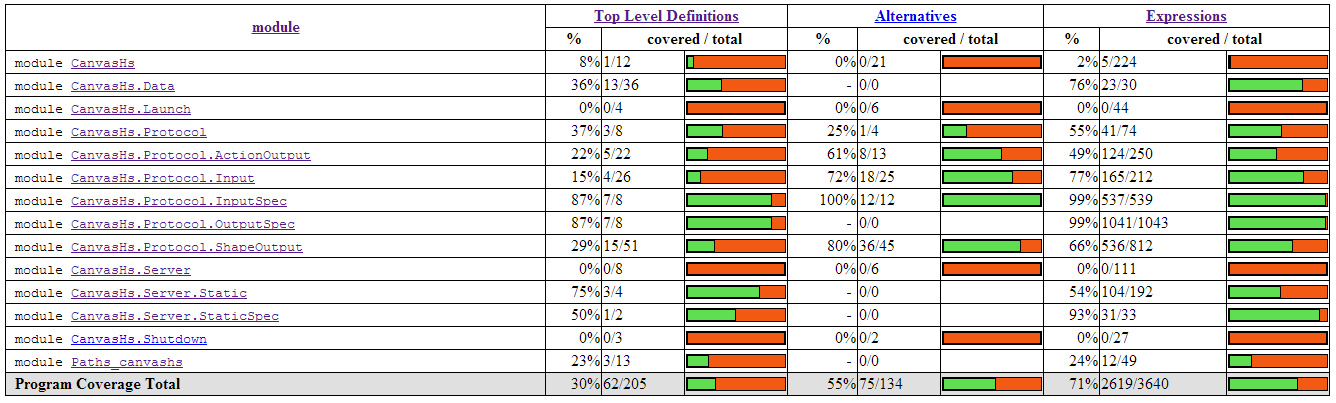
\includegraphics[keepaspectratio,width=\textwidth]{./images/haskellcoverage.png}
\caption{Code coverage resultaten uit HPC}
\label{fig:hpc}
\end{center}
\end{figure}

De code coverage resultaten die uit een analyse van HPC komen zijn niet direct uit te drukken in één compleet getal. Zoals te zien is in \autoref{fig:hpc}, zijn er verschillende onderdelen van de code die gemeten worden, namelijk: de definities, alternatieven en expressies. Bij het evalueren van de resultaten kijken wij naar de expressies van de modules die relevant zijn voor het gegevensmodel. Zo zijn de test-modules zelf meegenomen in de resultaten, maar deze zijn voor de resultaten niet relevant. Daarnaast zijn modules die te maken hebben met I/O en randzaken ook niet meegenomen in onze beoordeling aangezien het lastig is hiervoor betrouwbare tests te schrijven.

We kijken specifiek naar de \inlinecode{CanvasHs.Data}, \inlinecode{CanvasHs.Input}, \inlinecode{CanvasHs.Output}, \inlinecode{CanvasHs.ActionOutput} en \inlinecode{CanvasHs.ShapeOutput}. Hier komt het neer op 848 geteste expressies van de 1304. Dat is een resultaat van 65 \% code coverage voor de geschreven relevante Haskell-code.

\subsection{Gebruiksvriendelijkheid API}
Voor de gebruiksvriendelijkheid van de API hebben we requirements opgesteld. Dit zijn requirements die getoetst worden op het feit of de implementatie hieraan voldoet of niet, er is geen test voor uit te voeren.

\begin{enumerate}[label={T\arabic*}]
	\setcounter{enumi}{\value{startvaluetest}}
	\item \label{test:opzet:monadisch} Alle functionaliteit die aangeboden wordt door Canvas.hs aan de gebruiker maakt geen gebruik van monadische constructies en voldoen daarmee aan \ref{req:monadisch}.
	\item \label{test:opzet:modulair} Canvas.hs is modulair opgebouwd en bezit over voldoende documentatie zodat latere uitbreidingen makkelijk toegevoegd kunnen worden aan de code. Hierdoor voldoet Canvas.hs aan \ref{req:maintenance}.
\end{enumerate}

\subsection{Traceability matrix} \label{sec:traceability}
De traceability matrix laat zien of alle requirements getest zijn. Wanneer een requirement niet getest is betekent dit dat de functie niet ge\"implementeerd is of dat er geen test voor bestaat. Met de traceability matrix kan bijgehouden worden of alle functionaliteiten ge\"implementeerd zijn. Om de traceability matrix enigszins overzichtelijk te houden is slechts een deel van de testcases opgenomen in de matrix.

\begin{figure}
\begin{center}
\resizebox{\linewidth}{!}{\begin{tabular}{cc|c|c|c|c|c|c|c|c|c|c|c|c|c|c|c|c|c|c|c|c|c|c|c|c|c|c|c|c|c|c|c|c|c|}
\cline{3-29}
& & \multicolumn{27}{ |c| }{Requirements} \\ \cline{3-29}
& & \ref{req:prim}  &
\ref{req:circle} &
\ref{req:rect} &
\ref{req:lines} &
\ref{req:bezier} &
\ref{req:text} &
\ref{req:pictures} &
\ref{req:colors:lines} &
\ref{req:colors:fill} &
\ref{req:colors:fill:gradient} &
\ref{req:event:key} &
\ref{req:event:mouse} &
\ref{req:event:scroll} &
\ref{req:action:animate} &
\ref{req:zoom} &
\ref{req:action:prompt} &
\ref{req:action:fullscreen} &
\ref{req:action:localfiles} &
\ref{req:action:userfiles} &
\ref{req:errors} &
\ref{req:launchbrowser} &
\ref{req:reload} &
\ref{req:debug} &
\ref{req:multiplatform} &
\ref{req:performance} &
\ref{req:maintenance} &
\ref{req:coverage}  \\ \cline{1-29}
\multicolumn{1}{|c|}{\multirow{4}{*}{Tests}} & \ref{test:js:convert:rgbajson:rgba} 		&   &   &   &   &   &   &   &   &   &   &   &   &   &   &   &   &   &   &   &   &   &   &   &   &   &   &		 \\ \cline{2-29}
\multicolumn{1}{|c|}{} & \ref{test:js:execute:actions:displayfixed}						&   &   &   &   &   &   &   &   &   &   &   &   &   &   &   &   & X &   &   &   &   &   &   &   &   &   &		 \\ \cline{2-29}
\multicolumn{1}{|c|}{} & \ref{test:js:execute:actions:displayfluid}						&   &   &   &   &   &   &   &   &   &   &   &   &   &   &   &   & X &   &   &   &   &   &   &   &   &   &		 \\ \cline{2-29}
\multicolumn{1}{|c|}{} & \ref{test:js:execute:actions:opencontrol}						&   &   &   &   &   &   &   &   &   &   &   &   &   &   &   &   &   &   &   & X &   &   &   &   &   &   &		 \\ \cline{2-29}
\multicolumn{1}{|c|}{} & \ref{test:js:execute:actions:closecontrol}						&   &   &   &   &   &   &   &   &   &   &   &   &   &   &   &   &   &   &   & X &   &   &   &   &   &   &		 \\ \cline{2-29}
\multicolumn{1}{|c|}{} & \ref{test:js:parse:actions:fullscreen}							&   &   &   &   &   &   &   &   &   &   &   &   &   &   &   &   & X &   &   &   &   &   &   &   &   &   &		 \\ \cline{2-29}
\multicolumn{1}{|c|}{} & \ref{test:js:convert:rgbajson:rgba}							&   &   &   &   &   &   &   & X & X &   &   &   &   &   &   &   &   &   &   &   &   &   &   &   &   &   &		 \\ \cline{2-29}
\multicolumn{1}{|c|}{} & \ref{test:js:convert:rgbajson:rgba:alphazero}					&   &   &   &   &   &   &   & X & X &   &   &   &   &   &   &   &   &   &   &   &   &   &   &   &   &   &		 \\ \cline{2-29}
\multicolumn{1}{|c|}{} & \ref{test:js:convert:rgbjson:rgba} 							&   &   &   &   &   &   &   & X & X &   &   &   &   &   &   &   &   &   &   &   &   &   &   &   &   &   &		 \\ \cline{2-29}
\multicolumn{1}{|c|}{} & \ref{test:js:draw:line}, \ref{test:haskell:line}				& X &   &   & X &   &   &   &   &   &   &   &   &   &   &   &   &   &   &   &   &   &   &   &   &   &   &		 \\ \cline{2-29}
\multicolumn{1}{|c|}{} & \ref{test:js:draw:rect}, \ref{test:haskell:rect}				& X &   & X &   &   &   &   &   &   &   &   &   &   &   &   &   &   &   &   &   &   &   &   &   &   &   &		 \\ \cline{2-29}
\multicolumn{1}{|c|}{} & \ref{test:js:draw:polygon}, \ref{test:haskell:polygon}			& X &   &   &   &   &   &   &   &   &   &   &   &   &   &   &   &   &   &   &   &   &   &   &   &   &   &		 \\ \cline{2-29}
\multicolumn{1}{|c|}{} & \ref{test:js:draw:arc}, \ref{test:haskell:arc}					& X &   &   &   &   &   &   &   &   &   &   &   &   &   &   &   &   &   &   &   &   &   &   &   &   &   &		 \\ \cline{2-29}
\multicolumn{1}{|c|}{} & \ref{test:js:draw:circle}, \ref{test:haskell:circle}			& X & X &   &   &   &   &   &   &   &   &   &   &   &   &   &   &   &   &   &   &   &   &   &   &   &   &		 \\ \cline{2-29}
\multicolumn{1}{|c|}{} & \ref{test:js:draw:circle:alpha} 								& X & X &   &   &   &   &   &   &   &   &   &   &   &   &   &   &   &   &   &   &   &   &   &   &   &   &		 \\ \cline{2-29}
\multicolumn{1}{|c|}{} & \ref{test:js:draw:text}, \ref{test:haskell:text}				& X &   &   &   &   & X &   &   &   &   &   &   &   &   &   &   &   &   &   &   &   &   &   &   &   &   &		 \\ \cline{2-29}
\multicolumn{1}{|c|}{} & \ref{test:js:draw:container}, \ref{test:haskell:containers}	& X &   &   &   &   &   &   &   &   &   &   &   &   &   &   &   &   &   &   &   &   &   &   &   &   &   &		 \\ \cline{2-29}
\multicolumn{1}{|c|}{} & \ref{test:js:draw:container:clipping} 							& X &   &   &   &   &   &   &   &   &   &   &   &   &   &   &   &   &   &   &   &   &   &   &   &   &   &		 \\ \cline{2-29}
\multicolumn{1}{|c|}{} & \ref{test:js:mouse}, \ref{test:haskell:mouse}					&   &   &   &   &   &   &   &   &   &   &   & X &   &   &   &   &   &   &   &   &   &   &   &   &   &   &		 \\ \cline{2-29}
\multicolumn{1}{|c|}{} & \ref{test:js:mouse:draw} 										&   &   &   &   &   &   &   &   &   &   &   & X &   &   &   &   &   &   &   &   &   &   &   &   &   &   &		 \\ \cline{2-29}
\multicolumn{1}{|c|}{} & \ref{test:haskell:scroll} 										&   &   &   &   &   &   &   &   &   &   &   &   &   &   &   &   &   &   &   &   &   &   &   &   &   &   &		 \\ \cline{2-29}

\multicolumn{1}{|c|}{} & \ref{test:blackbox:keyevents}	 								&   &   &   &   &   &   &   &   &   &   & X &   &   &   &   &   &   &   &   &   &   &   &   &   &   &   &		 \\ \cline{2-29}
\multicolumn{1}{|c|}{} & \ref{test:blackbox:scrollevents}								&   &   &   &   &   &   &   &   &   &   &   &   & X &   &   &   &   &   &   &   &   &   &   &   &   &   &		 \\ \cline{2-29}


\multicolumn{1}{|c|}{} & \ref{test:blackbox:prompt}										&   &   &   &   &   &   &   &   &   &   &   &   &   &   &   & X &   &   &   &   &   &   &   &   &   &   &		 \\ \cline{2-29}
\multicolumn{1}{|c|}{} & \ref{test:blackbox:lokalebestanden}							&   &   &   &   &   &   &   &   &   &   &   &   &   &   &   &   &   & X &   &   &   &   &   &   &   &   &		 \\ \cline{2-29}
\multicolumn{1}{|c|}{} & \ref{test:blackbox:animatie}									&   &   &   &   &   &   &   &   &   &   &   &   &   & X &   &   &   &   &   &   &   &   &   &   &   &   &		 \\ \cline{2-29}
\multicolumn{1}{|c|}{} & \ref{test:blackbox:download}, \ref{test:haskell:download}		&   &   &   &   &   &   &   &   &   &   &   &   &   &   &   &   &   &   & X &   &   &   &   &   &   &   &		 \\ \cline{2-29}
\multicolumn{1}{|c|}{} & \ref{test:blackbox:upload} 									&   &   &   &   &   &   &   &   &   &   &   &   &   &   &   &   &   &   & X &   &   &   &   &   &   &   &		 \\ \cline{2-29}
\multicolumn{1}{|c|}{} & \ref{test:blackbox:error} 										&   &   &   &   &   &   &   &   &   &   &   &   &   &   &   &   &   &   &   & X &   &   &   &   &   &   &		 \\ \cline{2-29}
\multicolumn{1}{|c|}{} & \ref{test:blackbox:debug} 										&   &   &   &   &   &   &   &   &   &   &   &   &   &   &   &   &   &   &   &   &   &   & X &   &   &   &		 \\ \cline{2-29}
\multicolumn{1}{|c|}{} & \ref{test:blackbox:multiplatform} 								&   &   &   &   &   &   &   &   &   &   &   &   &   &   &   &   &   &   &   &   &   &   &   &   & X &   &		 \\ \cline{2-29}
\multicolumn{1}{|c|}{} & \ref{test:blackbox:browser} 									&   &   &   &   &   &   &   &   &   &   &   &   &   &   &   &   &   &   &   &   &   &   &   &   &   & X &		 \\ \cline{2-29}
\multicolumn{1}{|c|}{} & \ref{test:blackbox:coverage} 									&   &   &   &   &   &   &   &   &   &   &   &   &   &   &   &   &   &   &   &   &   &   &   &   &   &   & X	 	 \\ \cline{2-29}
\end{tabular}}
\caption{Traceability matrix, zie \autoref{sec:traceability}}
\label{fig:traceability}
\end{center}
\end{figure}






\section{Performance analyse} \label{sec:performance}

Tijdens de ontwikkeling van de library is duidelijk geworden dat de performance van de geschreven programma's niet altijd optimaal is. Met name bij programma's die gebruik maken van \emph{timers} en bij programma's met een uitgebreidde grafische boom.

Dit peformance probleem kan twee oorzaken hebben, ten eerste is het mogelijk dat de module van de applicatie niet snel genoeg JSON-berichten kan coderen en anderzijds is het mogelijk dat de client de binnengekomen berichten niet snel genoeg kan verwerken.

Eerst is gekeken naar de peformance van de module, hiervoor is voornamelijk gekeken naar het geheugengebruik gezien er het vermoeden was dat de module mogelijk te veel geheugen zou gebruiken (mogelijk door een geheugenlek) en voortdurend aan het garbage collecten is. Na een heap profile gemaakt te hebben bleek dat de Haskell code in totaal 600kb aan geheugen gebruikt, en dit getal stabiel is. De Haskell kant gaf dus geen problemen.

\subsection{Performance JavaScript-code}

De analyse van de client van Canvas.hs brengt een groter probleem aan het licht. In het ontwerp is ervoor gekozen de grafische boom stateless te maken. Dit betekend dat, zodra een nieuwe tekenactie door de module vertaald wordt, de client de hele grafische boom opnieuw doorgestuurd krijgt. In de client wordt deze grafische boom volledig opnieuw getekend. Hiervoor dient onder andere eerst een nieuwe \emph{stage} opgebouwd te worden.
Het opbouwen van de stage bleek erg kostbaar te zijn en duurde KineticJS ongeveer 6 ms (tegen 0.5 ms voor het opnieuw tekenen van dezelfde stage). Dit hebben is gemeten met de JavaScript-profiler in Google Chrome. De exacte getallen zijn niet direct interessant bij een CPU-profiel, de verhouding daarentegen wel. Het feit dat het opbouwen van de stage twaalf maal langer duurt dan het tekenen van het test programma bevestigd het probleem.

In \autoref{sec:aanbevelingen} wordt een aanbeveling gedaan voor het aanpakken van dit performance probleem. Hierin wordt voogesteld updates incrementeel uit te laten voeren waarbij niet bij elk bericht van de module de stage opnieuw opgebouwt hoeft te worden. Om dit te realiseren zal wel een groot deel van de code en hoogstwaarschijnlijk ook de API aangepast moeten worden.

\subsection{Performance Haskell-code}

In de module is een optimalisatie doorgevoerd die te maken heeft met het vertalen van strings naar verschillend types. Er was het vermoeden dat er in de Haskell-code van Canvas.hs veel peformance verloren zou gaan doordat we \inlinecode{Strings} naar \inlinecode{ByteStrings} naar \inlinecode{Text} vertaalde. Het bleek dat de laatste vertaalslag overbodig is, en daarom is deze verwijderd. Hieronder volgen twee grafieken, \autoref{fig:performance1} en \autoref{fig:performance2}~, die het geheugengebruik van de module van Canvas.hs demonstreren met en zonder de extra translaties.

Uiteindelijk blijkt deze wijziging weinig verschil gemaakt te hebben in het totale geheugengebruik. Desondanks was de optimalisatie niet voor niets gezien het de Haskell-code een stuk leesbaarder heeft gemaakt. Wel is te zien dat in het eerste figuur de garbage collecting van Haskell aggresiever lijkt, dus wellicht wordt zonder de wijziging toch meer memory tijdelijk gebruikt en vervolgens direct weer vrijgegeven. Verder valt op dat na de optimalisatie er toch \inlinecode{Text} in de heap profile staat. Dit is vermoederlijk omdat een van de libraries die gebruikt wordt door Canvas.hs daar intern gebruik van maakt.

Voor dit specifieke geval zijn de heap profiles niet interessant, het grootste gedeelte van de data is \emph{PINNED} data, dit zijn vooral \inlinecode{ByteString} allocaties. Gezien de module vooral een translator is van het protocol naar een aantal \inlinecode{ByteStrings} is dit niet verrassend. Wel bieden dit soort grafieken duidelijk inzicht in of er geheugenlekken zijn en of er onnodige conversies gemaakt worden, voor grote projecten zijn dit soort grafiekjes zeker nuttig.

\begin{figure}[H]
\begin{center}
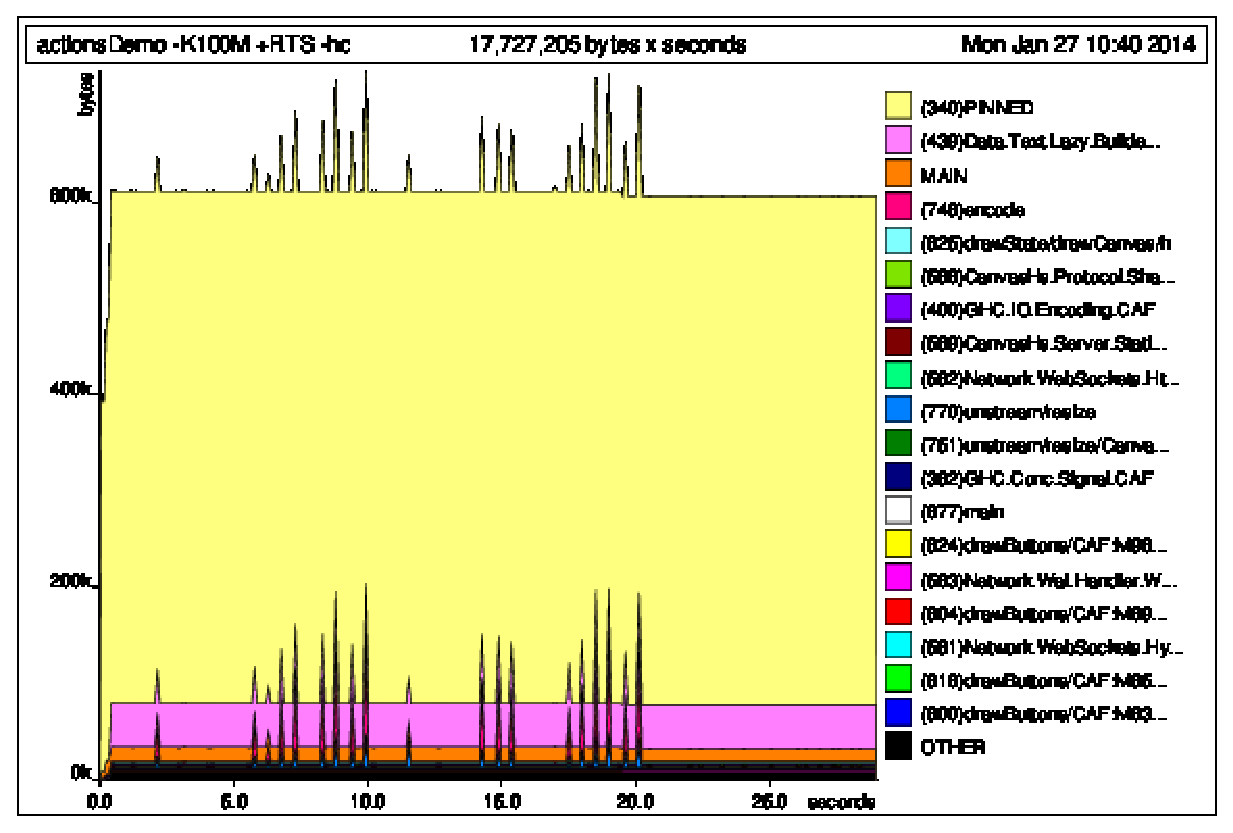
\includegraphics[keepaspectratio,width=0.8\textwidth]{./images/actionsDemoBeforeByteStrings.eps}
\caption{Heap profile voor de wijziging}
\label{fig:performance1}
\end{center}
\end{figure}

\begin{figure}[H]
\begin{center}
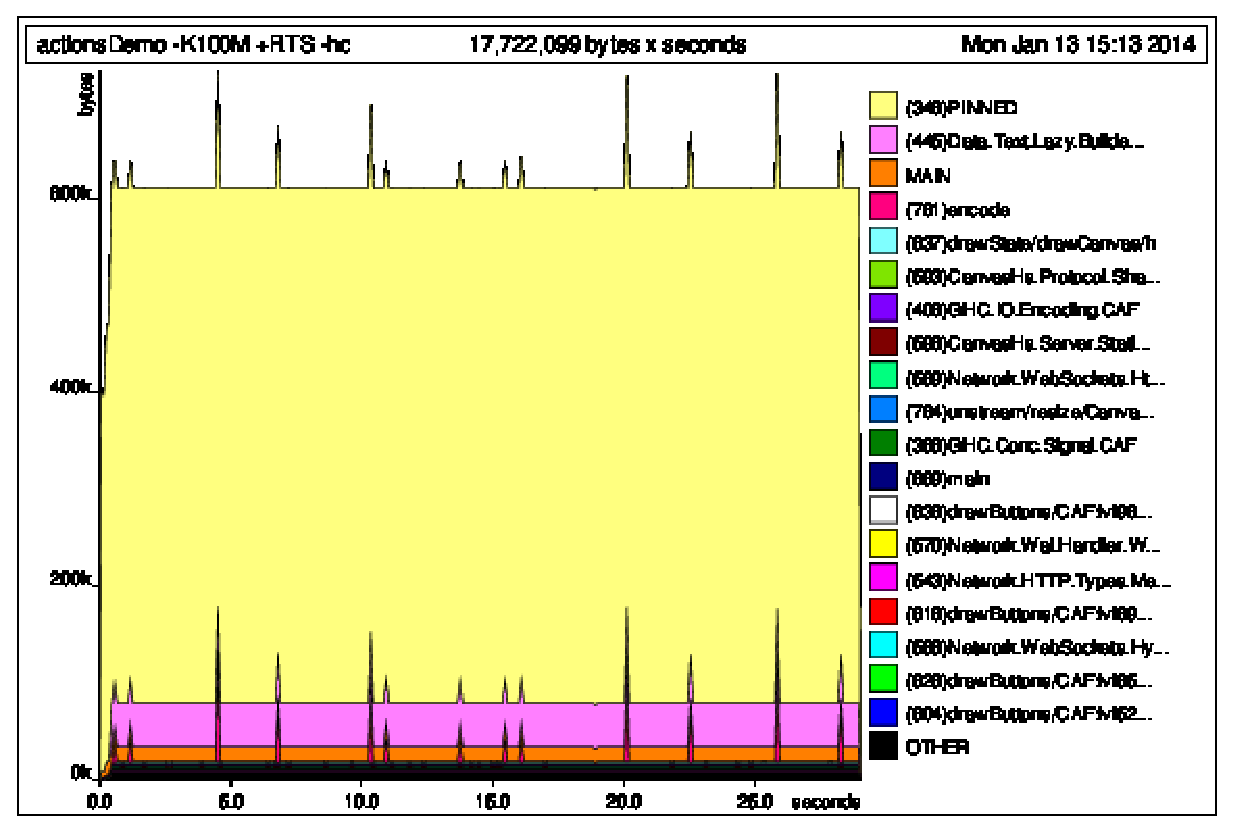
\includegraphics[keepaspectratio,width=0.8\textwidth]{./images/actionsDemoAfterByteStrings.eps}
\caption{Heap profile na de wijziging}
\label{fig:performance2}
\end{center}
\end{figure}

\chapter{Evaluatie} \label{hoofdstuk:evaluatie}
\todo{evaluatie tenopzichte van de requirements}
\section{Verbeteringen en aanbevelingen}
\subsection{Delta updates (met animaties)}

\section{Problemen}
\subsection{IO Monad afsplitsen}

{\color{red} Onderstaande had ik (Pim) origineel geschreven voor het problemenstuk (in ontwerp), he tmoet nog aangevuld/afgemaakt worden e.d., maar dat is iets wat bij evaluatie kan. Het is over de problemen die we hadden omdat we relatief weinig haskell-kennis hadden}

\subsubsection{Kennis Haskell}
Bij het begin van het Canvas.Hs-project was de kennis over Haskell en functioneel programmeren in het algemeen beperkt tot de kennis opgedaan met het vak Functioneel programmeren. Hoewel dit een solide basis vormt is het doel van Canvas.Hs juist om een aantal concepten die niet binnen dit vak passen af te schermen van de studenten. Dit betekende dat er bij het project van deze concepten gebruik moest worden gemaakt en wij ons deze ook eigen hebben moeten maken. Zoals altijd bij het leren van nieuwe concepten leverde dit af en toe code die niet optimaal gebruik maakte van de mogelijkheden van deze concepten en kinderziektes op. 

Naarmate het project vorderde vorderde ook onze kennis van Haskell, hierdoor maakt de uiteindelijke versie van Canvas.Hs goed gebruik van de mogelijkheden van o.a. monadisch programmeren en Haskells threadsysteem. 
\paragraph{Monads}
Zoals gezegd kent Haskell het concept van monads. Één van de doelen van CanvasHs is om dit concept niet te hoeven gebruiken voor grafische weergave bij het vak functioneel programmeren. Dit betekent dat ook wij, de ontwikkelaars, weinig kennis over dit concept hadden voor aan het project begonnen werd. Doordat we 
Denk aan do-notatie, binds (>>=
>>) en eigen monad voor de Server (state)
\todo{onvoldoende toegelicht}

\paragraph{Threads}
Denk aan geziek met netjes de WebSockets en http-threads afsluiten en Timer-threads die nu doorlopen

\section{Planning}
\todo{Planning schrijven}
\section{Samenwerking}
\todo{Dit moet naar het begin van het verslag}
Tijdens het ontwikkelen van de eerste versie van Canvas.HS is er samengewerkt volgens een paar vooraf geselecteerde methoden. Zo zijn er onderdelen van de Scrum projectmanagement methode gebruikt alsmede andere Agile methoden.

De samenwerking is goed verlopen. Daarbij was de duidelijke structuur van zowel het project– als de technische organisatie een belangrijk onderdeel. Er kon met deze structuur, naar gevoel van de projectgroep, efficiënt gewerkt worden. Er werd wekelijks twee of meer keer samengekomen om te werken aan het project.

\subsection{Project organisatie}
Er is gewerkt middels de scrum projectmangement methoden. Er is gewerkt met verschillende rollen en er zijn zogenaamde scrum en sprint besprekingen gehouden. Daarbij zijn elke keer opnieuw onder andere het project– en sprintbacklog samengesteld en bijgewerkt.

\paragraph{Rollen} Er is een verdeling van verantwoordelijkheden gemaakt. Naast de teamleden nam de opdrachtgever de rol van \emph{product owner} aan.
\begin{enumerate}
    \item \emph{J. van Doorn} had de taak van \emph{scrum master} en was verantwoordelijk voor het testen van de software.
    \item \emph{P.T. Jager} was notulist voor alle besprekingen en samen met Buit verantwoordelijk voor de Haskell code.
    \item \emph{L.J. Buit} was verantwoordelijk voor het protocol en samen met Jager verantwoordelijk voor de Haskell code.
    \item \emph{M.J. Roo} was samen met Scheepers verantwoordelijk voor de JavaScript code.
    \item \emph{M.J. Scheepers} was verantwoordelijk voor de gebruiksvriendelijkheid uiteindelijke API en samen met Roo verantwoordelijk voor de JavaScript code.
\end{enumerate}

\paragraph{Besprekingen} Elke samenkomst is er een kortdurende scrumbespreking gehouden. Na aanvang van het project zijn er ook een aantal sprint besprekingen gehouden. Deze sprint besprekingen kwamen altijd na het gesprek met de opdrachtgever. Er bleek al snel dat onze afgesproken sprint van twee werken wel erg kort was om elke twee weken dat er samengekomen werd een nieuwe lange sprintbespreking te houden. Dus er werd uiteindelijk voor gekozen om de besprekingen met de projectgroep te beperkingen tot de dagelijkse korte besprekingen.

Bij de dagelijkse besprekingen werd vaak op details in gegaan, hierbij werden ontwerp beslissingen vaak genomen tijdens deze besprekingen. De besprekingen duurde hierdoor soms wat lang en werden zittend gehouden.

\paragraph{Taken}
Regelmatig werd de lijst met taken bijgewerkt. Taken bestonden uit: projecttaken, als het bijhouden van de planning; ontwikkeltaken, als het oplossen van bugs en het schrijven van nieuwe features; schrijftaken en overige taken.

\begin{figure}[H]
\begin{center}
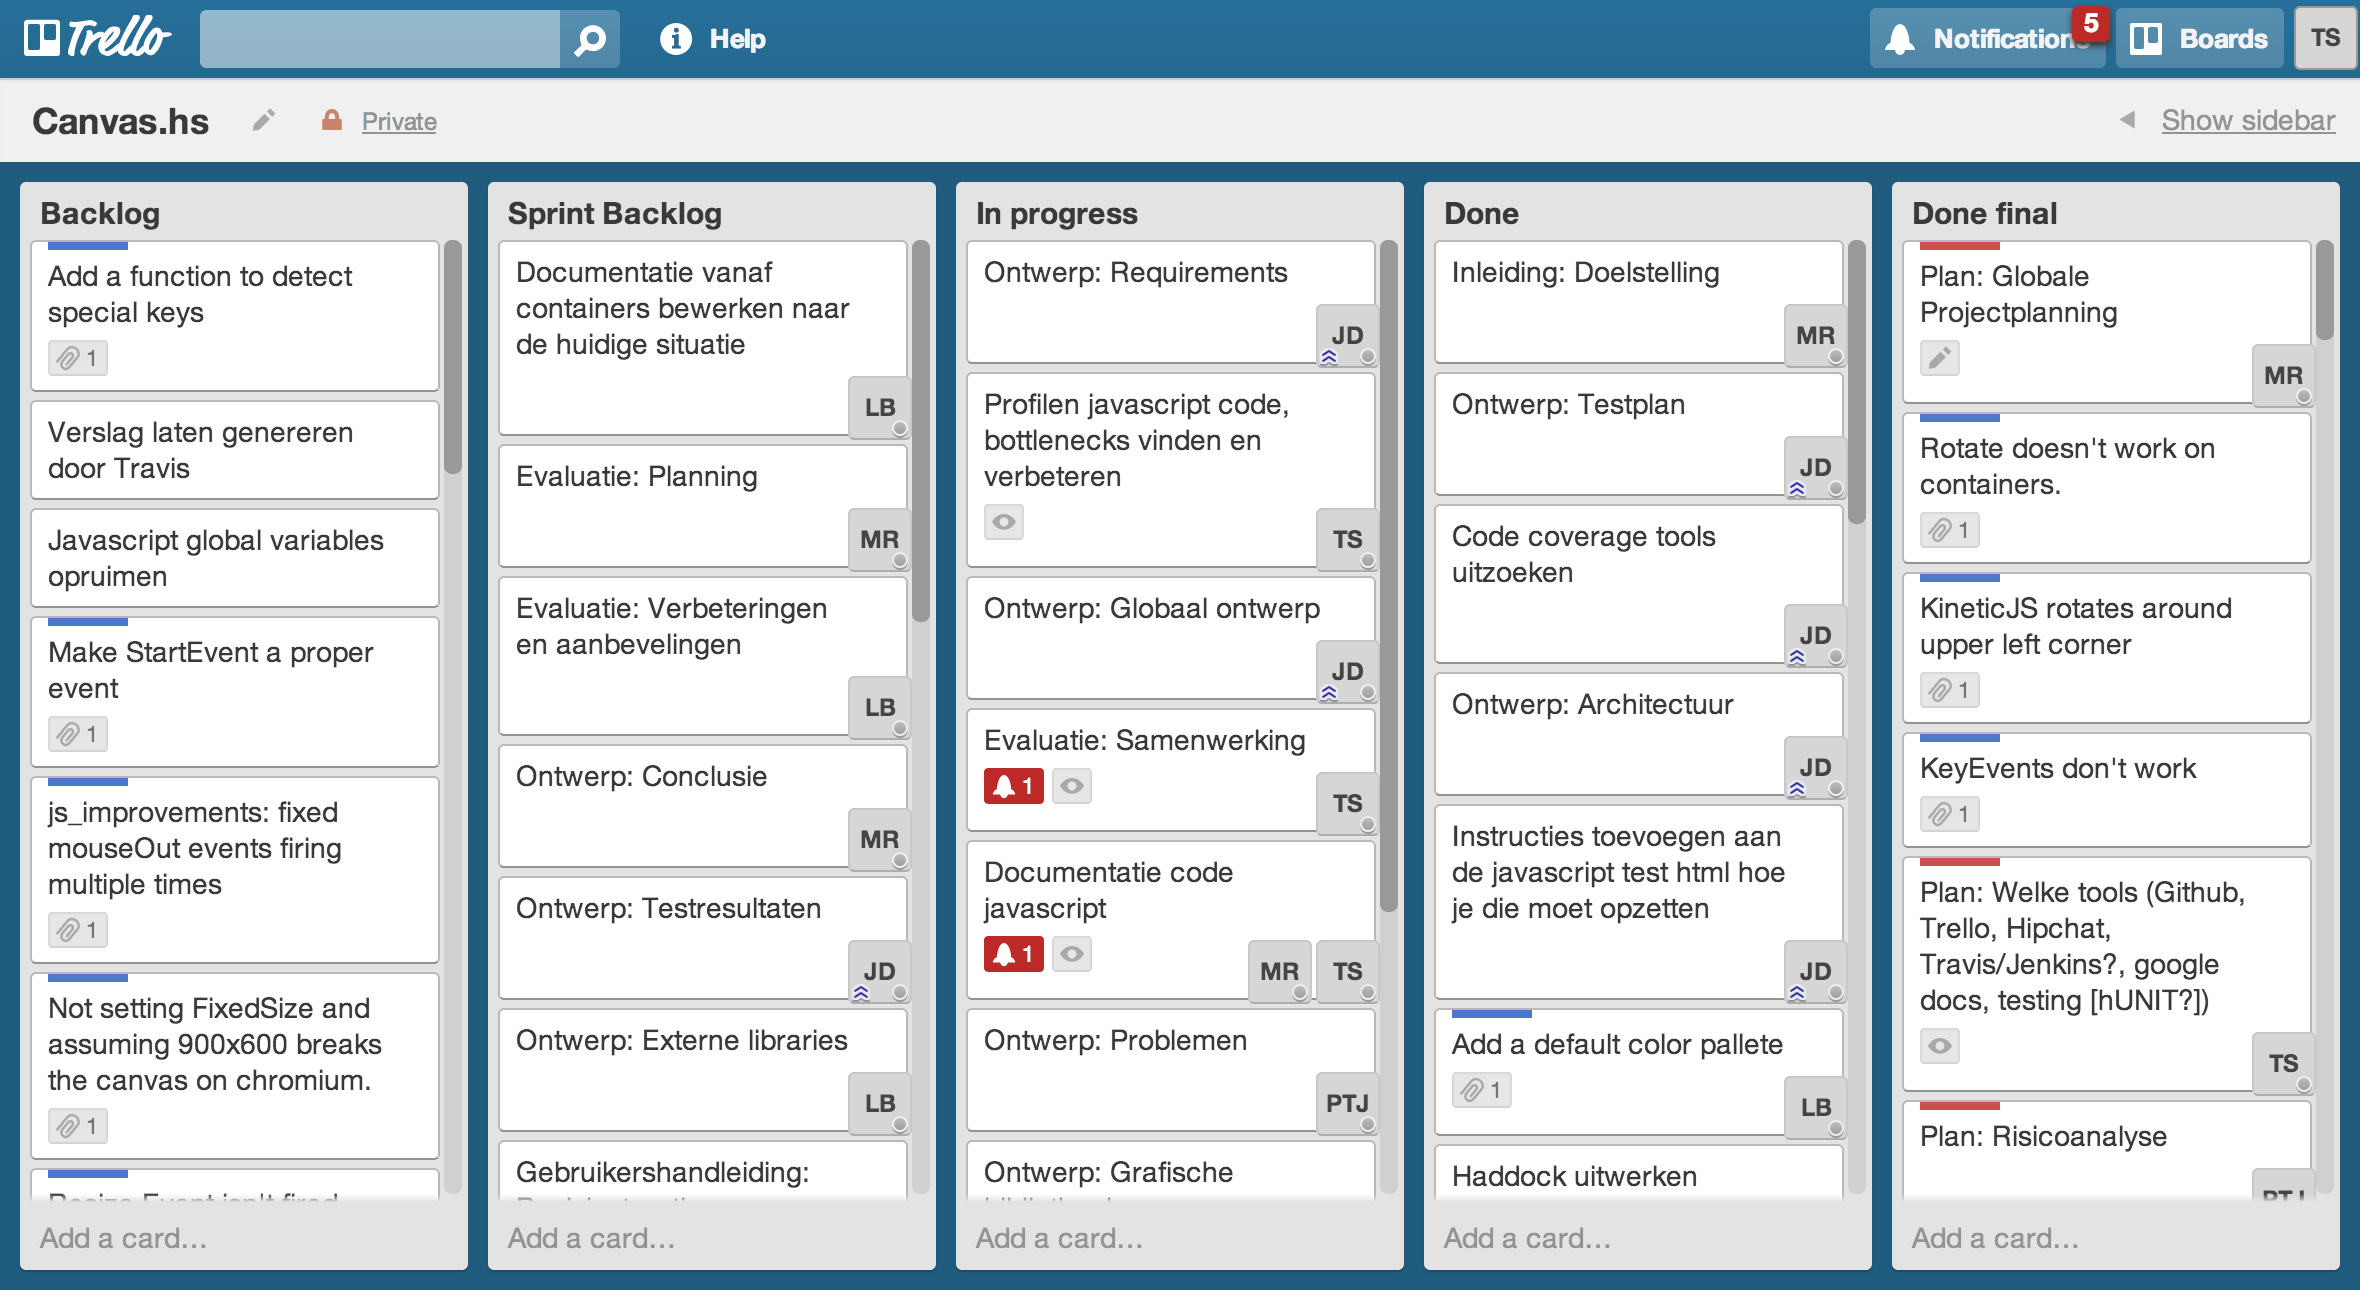
\includegraphics[keepaspectratio,width=\textwidth]{./images/trello.png}
\caption{Trello board}
\label{fig:trello}
\end{center}
\end{figure}

De lijst van ontwikkeltaken werd bijgehouden op het \emph{GitHub} platform. Deze taken werden daar ook wel Issues genoemd. Andere taken werden vervolgens bijgehouden op \emph{Trello}. Met deze applicatie kan een online takenbord gemaakt worden, zie \autoref{fig:trello}. De ontwikkeltaken werden middels synchronisatie ook op dit takenbord gezet. Door \emph{Trello} had elk lid van het project een goed inzicht in de taken die nog openstonden en reeds waren uitgevoerd.

\paragraph{Terugkoppeling naar de opdrachtgever} De opdrachtgever—binnen scrum ook \emph{product owner} genoemd—is twee wekelijks ge\"informeerd over de voortgang. De terugkoppeling die de opdrachtgever gaf werd besproken en verwerkt in de volgende versie van de library.

\paragraph{Verbeteringen} Er is nu gewerkt in een projectgroep zonder direct uren budget, mocht dit het geval zijn zouden de inschattingsmethoden en burndown chart uit de scrum methode kunnen worden gebruikt. Verder zouden de besprekingen zogenaamde \emph{stand-up meetings} kunnen worden waarbij iedereen staat en niet voor de computer zit. Hierdoor konden de dagelijkse besprekingen wellicht wat vlotter verlopen.

\subsection{Versiebeheer}
Bij het bouwen van software met een groep is het belangrijk dat een ontwikkelaar zich kan concentreren op de feature die hij aan het ontwikkelen is. Idealiter hoeft er geen rekening gehouden te worden met andere features die door anderen ontwikkeld worden. Er is dan ook gekozen om gebruik te maken van het gedistribueerde versiebeheer systeem \emph{Git} met een centraal repository op \emph{GitHub}.

Over het gebruik van deze software zijn afspraken gemaakt. Zo is er gebruik gemaakt van verschillende \emph{branches}. Als een bepaalde versie van de software op een bepaalde branch staat zegt dit iets over de status van die versie. Zo kan er begonnen worden aan een nieuwe feature vanaf de \inlinecode{dev} branch. En is een versie op de \inlinecode{master} branch klaar voor gebruik.

\paragraph{Feature branches en pull requests}
Bij aanvang van de ontwikkeling van een nieuwe feature werd er een nieuwe branch gemaakt vanaf de \inlinecode{dev} branch. Een voorbeeld hiervan is de \inlinecode{arcs} branch. In \autoref{sec:shapesext} staat beschreven hoe \inlinecode{Arc} shapes toegevoegd kunnen worden. Dit is dus gebeurd op een aparte branch die begonnen is vanaf de \inlinecode{dev} branch, zie \autoref{fig:pullrequest}. 

\begin{figure}
\begin{center}
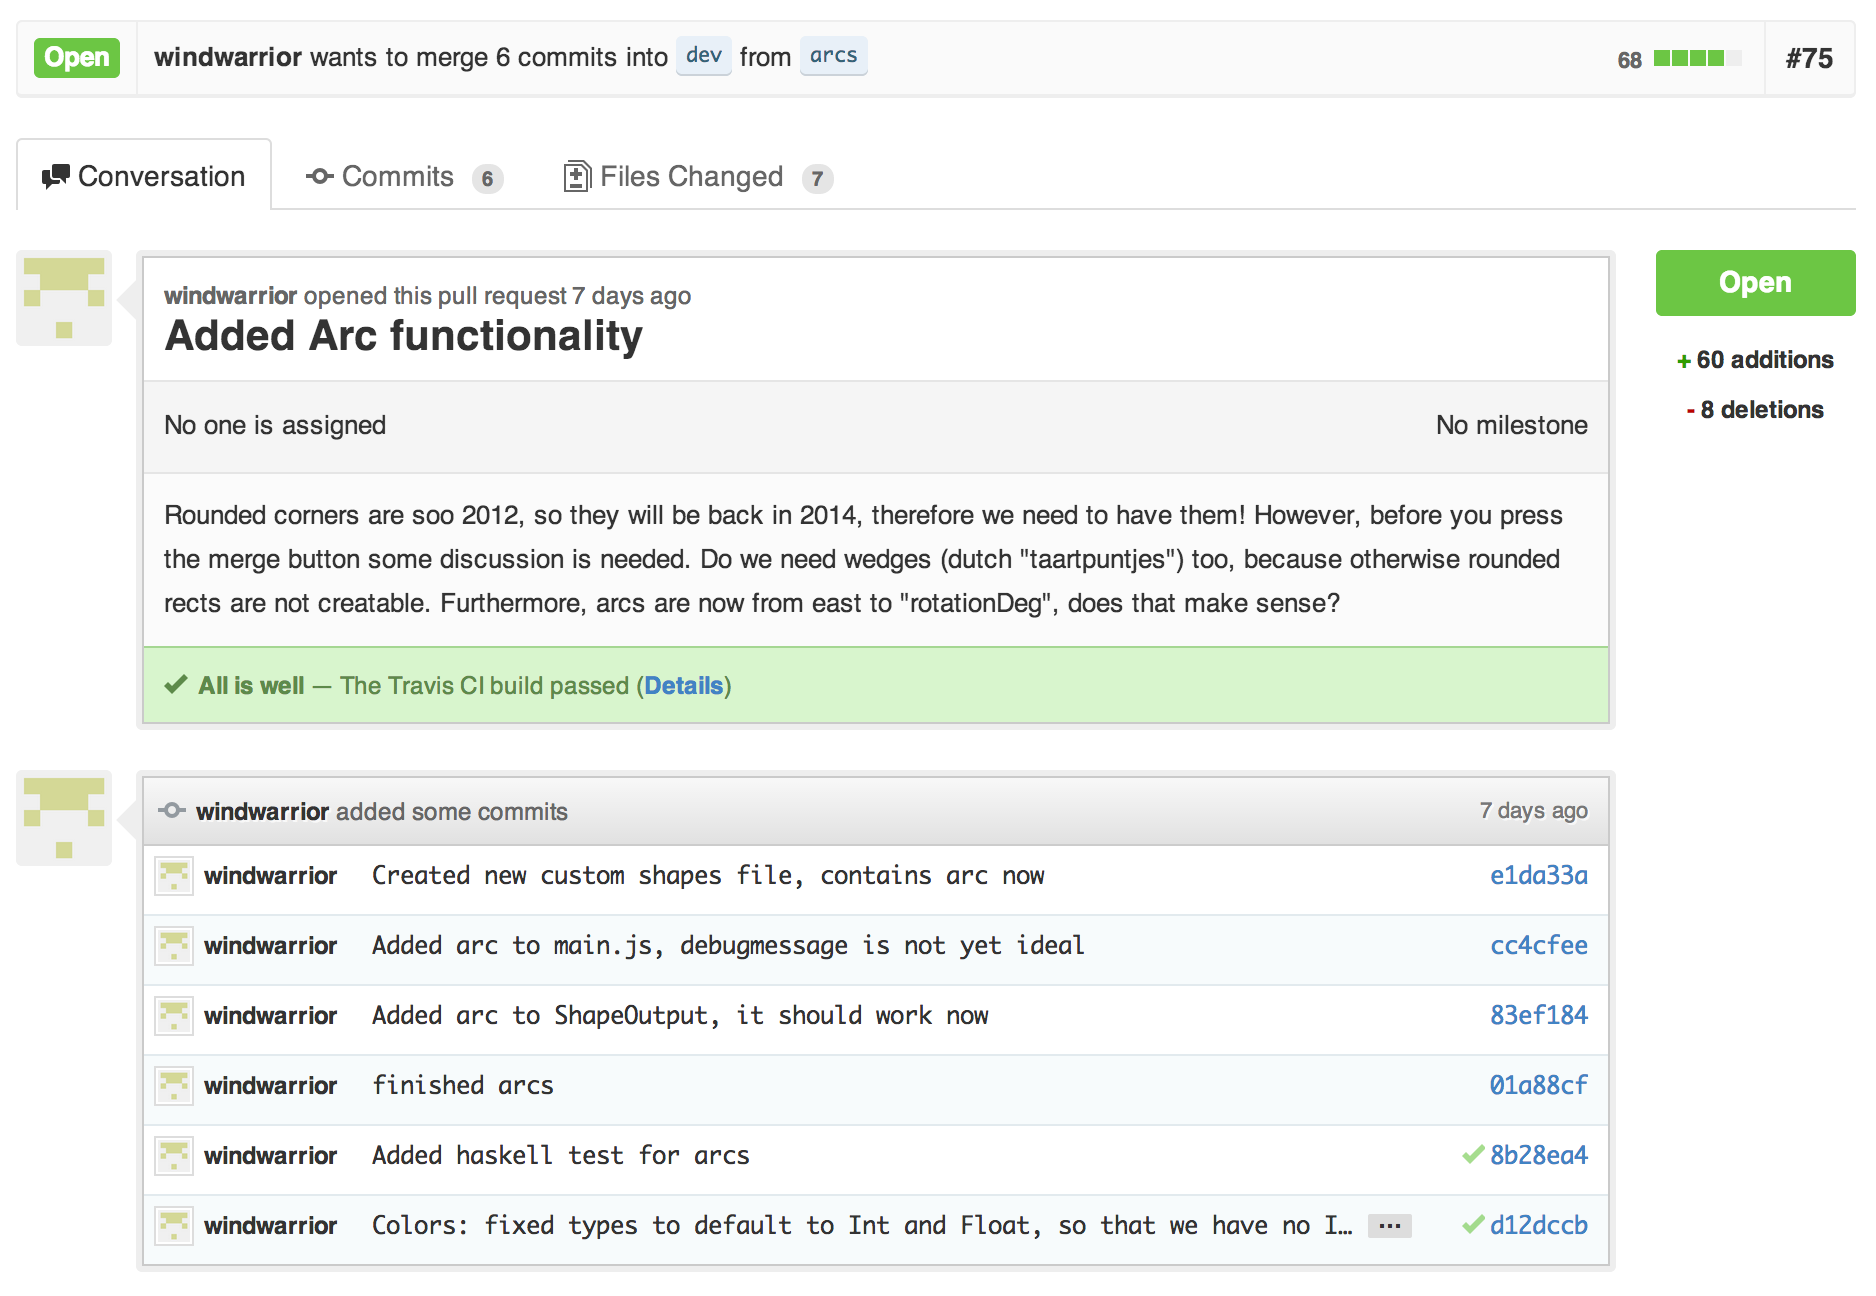
\includegraphics[keepaspectratio,width=\textwidth]{./images/pullrequest.png}
\caption{Pull Request \#75 Arcs geimplementeerd. – \url{https://github.com/CanvasHS/Canvas.hs/pull/75}}
\label{fig:pullrequest}
\end{center}
\end{figure}

Als een feature af is moet deze beoordeeld voordat deze gemergd kan worden naar de \inlinecode{dev} branch. Daarvoor wordt een \emph{pull request} aangemaakt. Deze \emph{pull request} bevat dan informatie over de wijzigingen tenopzichte van de versie die op de \inlinecode{dev} branch staat. Een beoordelaar kan de code lezen en deze goedkeuren. Op het moment dat de code goed wordt gekeurt komt een nieuwe versie met de nieuwe feature op de \inlinecode{dev} branch te staan.

Bij aanvang van het project was deze werkwijze voor veel teamleden nieuw. En daarom is het in het begin niet altijd juist toegepast. Maar naarmate het project vorderde is steeds vaker met succes gebruik gemaakt van het pull request principe. Dit zorgde er voor dat teamleden elkaars code controleerde en dat er minder bugs zaten in de versies op de \inlinecode{dev} branch.

\paragraph{Continuous integration} Om het beoordelen van code gemakkelijk te maken voor de ontwikkelaar en de beoordelaar is er gebruik gemaakt van de \emph{continuous integration} software \emph{Travis}. Deze software luistert naar nieuwe commits naar het centrale repository, als er een nieuwe commit gedaan is wordt er een virtuele machine opgestart die vervolgens middels een buildscript de versie van de software probeert te bouwen. Dit buildscript staat in de root directory van het repository.

Dit buildscript specificeert onder andere dat de software gebouwd moet worden met de Haskell compiler, maar ook dat alle geschreven tests uitgevoerd moeten worden. Mocht de compilatie of het uitvoeren van een van de tests niet geslaagd zijn is de build gefaald. Dit wordt dan vervolgens ook weergeven in het venster van de pull request. Als een beoordelaar ziet dat de build uit een pull request succesvol is, zoals bijvoorbeeld te zien bij \autoref{fig:pullrequest}, weet hij zeker dat de versie veilig is om te mergen.

Het buildscript voert naast de compilatie en de testen nog een paar andere commando's uit. Zo genereert het buildscript ook de documentatie en uploadet deze naar de Canvas.HS website—\url{http://canvashs.github.io}. Op de website kan de documentatie bekeken worden per build. Hierdoor hoeven ontwikkelaars zelf geen documentatie meer te genereren en hebben zij altijd, up to date, doorzoekbare documentatie.

\paragraph{Verbeteringen} Naast het integreren van documentatie zou het buildscript ook automatisch per versie de test coverage uit kunnen rekenen. Dit zou ontwikkelaars nog meer inzicht kunnen geven in de kwaliteit van de software en hoe deze voor– of achteruit gaat per versie.

 
% !TEX spellcheck = nl_NL
\chapter{Conclusie \& Toekomstig werk} \label{hoofdstuk:conclusie}
Dit project had als doel om een nieuwe omgeving te ontwikkelen die beginnende Haskell-programmeurs, zoals studenten van het vak Functioneel Programmeren, in staat stelt om grafische weergaven te maken en te manipuleren met eenvoudige, zelfgeschreven Haskell-code. Deze omgeving zou bovendien op alle gangbare platformen moeten draaien terwijl de installatie van de omgeving niet onredelijk ingewikkeld moest zijn.

Canvas.hs, de ontwikkelde omgeving die in dit verslag gepresenteerd is, is de vervulling van dit doel. 

In \autoref{hoofdstuk:requirements} staan de requirements die aan de ontworpen omgeving gesteld werden en de traceability matrix in \autoref{sec:traceability} geeft aan welke requirements door welke tests geverifieerd worden.

\todo{Voltooi Conclusie}

Hieronder worden aspecten besproken die nog missen in Canvas.hs. Ook wordt per aspect aangegeven hoe ondersteuning voor die aspect toegevoegd kan worden in toekomstige versies.

\section{Aanbevelingen}

\subsubsection{Image type}
Canvas.hs ondersteunt een breed scala aan grafische primitieven, zo goed als alle vectortekeningen zijn te maken met deze library. Helaas mist er ondersteuning voor plaatjes, zo kan de gebruiker bijvoorbeeld geen fotoalbum in Haskell/Canvas.hs schrijven.

Het toevoegen van een \inlinecode{Image} type is daarentegen redelijk triviaal, al zal er nog wel over peformance nagedacht moeten worden. De eerste optie is dat de gebruiker het plaatje inleest (middels de \inlinecode{LoadFileBinary}) en vervolgens een \inlinecode{Image} node toevoegt die als argument een ByteString neemt, en dit aanbiedt aan Canvas.hs. Een andere optie is de foto te serveren vanuit de server, dus de gebruiker moet een image in een bepaalde map zetten, en de webserver serveert dat image dan op een statische manier.

Een groot nadeel aan de eerste methode is dat het plaatje steeds opnieuw naar base64 gedecodeerd moet worden, en over de socket gestuurd moet worden. Verder moet de gebruiker de bytestring van het plaatje bewaren, ander zou die steeds opnieuw ingeladen moeten worden. De tweede methode is flexibeler, Canvas.Hs stuurt alleen een locatie op naar de client, en de client kan zelfs cachen waar de foto opgeslagen is. Helaas betekent dit wel dat de gebruiker de foto waarschijnlijk in een specifiek mapje moet plaatsen.

Het implementeren van nieuwe shapes wordt in een van de appendices uitgebreid besproken.

\subsubsection{Kleurverlopen}
Binnen Canvas.hs kan tot op heden alleen met vaste keuren gevuld worden, voor het tekenen van knoppen is het vaak gewenst iets van een kleurverloop te gebruiken. Een kleurverloop kan namelijk diepte bieden aan een grafisch element. Het ondersteunen van kleurverlopen is ook niet lastig, de clientside Javascript library (Kinetic) ondersteunt al kleurverlopen, dus het is een kwestie van het toevoegen en implementeren van een API voor de gebruiker.

\subsubsection{Grafische toolkit}
\subsubsection{Delta updates}
Op dit moment wordt de client behandeld alsof het stateless is, de module stuurt na elke verandering de hele grafische boom op en de client gooit zijn hele interne boom weg en accepteerd de nieuwe. Deze manier van werken is vanuit een Haskell oogpunt logisch, maar door het gebrek aan caching is het in Javascript traag. Daartoe is het handig om delta updates te sturen, zo kan er opgestuurd worden dat een rondje drie keer zo groot geworden is. Helaas is dit nog niet triviaal, er moet bijvoorbeeld rekening gehouden worden met identieke nodes (bijvoorbeeld een cirkel op (0,0) met radius 10)
\subsubsection{FPprac module}


\newpage
\appendix
\newcommand{\myparagraph}[1]{\paragraph{#1}\mbox{}\\}
% commando's om het invoegen van een aantal vaak voorkomende woorden gemakkelijker te maken
\newcommand{\type}[1]{\inlinecode{#1}}
\newcommand{\events}{\type{Event}'s\xspace}
\newcommand{\actions}{\type{Action}'s\xspace}
\newcommand{\shapes}{\type{Shapes}'s\xspace}
\newcommand{\shape}{\type{Shape}\xspace}



%commando's om een aantal vaak voorkomende wooden makkelijker te maken
\newcommand{\events}{\lstinline{Event's}\xspace}
\newcommand{\actions}{\lstinline{Action's}\xspace}
\newcommand{\shapes}{\lstinline{Shapes's}\xspace}
\newcommand{\type}{\lstinline}
\newcommand{\shape}{\type{Shape}\xspace}



\chapter{Gebruikerhandleiding} \label{sec:gebruikershandleiding}

%TODO: een appendix package oid gebruiken

\section{Inleiding}

Canvas.hs is een Haskell bibliotheek om op een simpele manier grafische elementen vanuit een Haskell programma weer te geven en te reageren op input vanuit de gebruiker. Met behulp van een webbrowser, met JavaScript en canvaselement worden de primitieven getekend, en wordt op gebruikersinput gereageerd.

Canvas.hs maakt het mogelijk om interactie te hebben met de gebruiker, het bestandssysteem en andere elementen uit de zogenaamde ``echte wereld'' zonder gebruik te hoeven maken van de IO Monad. Op deze manier is het voor beginnende Haskell-programmeurs mogelijk om grafische programma's te schrijven zonder begrip te hebben van monads en monadische computaties.

Om dit alles te bereiken wordt gebruik gemaakt van event-driven-IO. De programmeur schrijft een handler-functie die elk event (bijvoorbeeld een klik van de gebruiker) afhandelt en daaruit een nieuwe output (bestaande uit een aantal te tekenen objecten en uit te voeren acties) oplevert. De bibliotheek maakt het daarnaast mogelijk voor de handler om een state bij te houden en deze bij elk event te lezen en aan te passen. 

Kort gezegd maakt canvas.hs het volgende mogelijk:
\begin{itemize}
	\item Grafische programma's schrijven in Haskell
	\item Reageren op input, zoals muisklikken en toetsaanslagen
	\item Interactie met het bestandssysteem, door bijvoorbeeld bestanden te lezen of op te slaan.
	\item Meer, zoals het gebruik van klokken en het sturen en ontvangen van bestanden uit de browser.
\end{itemize}
Dit alles zonder gebruik te hoeven maken van monadisch programmeren. 

In deze gebruikershandleiding zal worden toegelicht hoe met behulp van Canvas.hs een grafisch haskellprogramma geschreven kan worden. Er zullen een aantal simpele voorbeelden gegeven worden, vervolgens zullen alle mogelijke te tekenen vormen (\shapes), uit te voeren acties (\actions) en te verwachten events (\events) uitgebreid worden toegelicht. 

\paragraph{Definities} 
Een tweetal begrippen uit deze handleiding verdienen nog even aandacht. Allereerst wordt de lezer van de handleiding aangesproken, hiermee wordt de programmeur bedoeld, degene die de handler schrijft en met de Canvas.Hs bibliotheek werkt. Daarnaast wordt gesproken over de \emph{Gebruiker}, dit is de persoon die interactie met het programma heeft via de canvas.

\section{Basisinstructies}

Om een Canvas.hs-applicatie te schrijven moeten we een handlerfunctie schrijven die events afhandelt. Een handlerfunctie heeft als type \inlinecode{handler :: a -> Event -> (a, Output)}. De \inlinecode{a}'s in dit signatuur zijn \inlinecode{State}'s. Elke keer dat de library een event binnenkrijgt zal onze handlerfunctie aangeroepen worden met de laatste state. Zoals de typesignatuur laat zien, zijn we verplicht deze state terug te geven zodat Canvas.hs hem op kan slaan.

\subsection{Termen}
Binnen deze handleiding zullen we een aantal termen gebruiken.
\begin{description}
	\item[Output]
De programmeur is verandwoorderlijk voor het produceren van output, meestal zal de programmeur een Shape en een lijst van Actions geven maar ook een BlockingAction is mogelijk.
	\item[Shape]
Binnen Canvas.hs is vrijwel alles een shape, maar binnen deze handleiding zal er onderscheid gemaakt worden tussen primaire shapes (Circle, Rect, etc.), containers (een shape die een aantal kinderen heeft) of modifiers (bewerkingen op een shape).
	\item[Modifiers]
Modifiers zijn bewerkingen op een Shape, zo is Rotate een modifier. Karaktiristiek aan een modifier is dat het als argument een shape neemt.
	\item[Containers]
Containers zijn shapes die meerdere shapes kunnen bevatten, zo kan de programmeur elementen groeperen.
	\item[Action]
Soms zal de programmeur een IO-bewerking willen uitvoeren, zoals het downloaden van een file. Dit is binnen Canvas.hs gemodelleerd als een Action.
	\item[BlockingAction]
Er zijn bepaalde acties die de uitvoer van het programma blokkeren, zoals het laden van een bestand. Het belangrijkste voor de programmeur is dat het niet mogelijk is om zowel een BlockingAction als een Shape terug te geven. 
    \item[Defaults]
Sommige elementen in de grafische boom bevatten veel mogelijkheden, zo kan tekst een ander font hebben, een andere grootte, schuin staan, dik zijn, etc. Daarom zijn er defaults gemaakt, dit is een functie die een aantal standaardwaarden teruggeeft. Voor tekst is dit bijvoorbeeld Arial, 12 pixels groot, niet bold of schuin en links uitgelijnd.
\end{description}

\subsection{Canvas.hs 101}
Om te beginnen introduceren we hier eerst een voorbeeld van een programma dat een rondje tekent. Zoals hierboven uitgelegd moet eerst een handler gedefinieerd worden. Deze zal zijn state samen met een output moeten teruggeven.

\lstinputlisting[style=densecode]{Examples/CanvasHs101.hs}

In het voorbeeld wordt een handler gemaakt. Deze eventHandler registreren we bij Canvas.hs met de functie installEventHandler. Deze eventHandler wordt aangeroepen als er een event plaatsvind. Als Canvas.hs dan een StartEvent vuurt (dit event vindt plaats als de servers succesvol gestart en verbonden zijn, zie \fullref{sec:handleiding_primitieven}), moet onze handler een state en een output teruggeven. Als state is een simpele integer gekozen en de output is in dit geval slechts een Shape. Deze code tekent een zwarte cirkel met radius 50 op punt (200,200).

Dit voorbeeld heeft geen modifiers, er zijn geen Shapes die werken op andere shapes. Daarnaast zijn er in dit eenvoudige voorbeeld geen Actions gebruikt. Er wordt uit de module CanvasHs wel een functie shape gebruikt, deze hulpfunctie returnt alleen een shape zonder acties en is daarmee gelijk aan \inlinecode{(Just shape, [])}.

% !TEX spellcheck = nl_NL
\section{Primitieven} \label{sec:handleiding_primitieven}
Nu we hebben gezien hoe we op verschillende \events kunnen reageren, en hoe we op basis daarvan \type{Output} kunnen genereren in de vorm van \shapes en \actions is het tijd om een volledig overzicht te geven van alle mogelijke \events , \shapes , en \actions.

Vergeet hierbij niet, zoals in het vorige hoofdstuk besproken, de types die belangrijk zijn voor Canvas.hs:

\begin{lstlisting}
-- Je functie die inkomende events afhandelt, State is hierbij een zelf te definiëren (data)type.
handler :: State -> Event -> (State, Output)

-- zie voor de verschillende Events hieronder
data Event = ...
		deriving(Eq, Show)

data Output = Block BlockingAction | Out RegularOutput

--zie voor de verschillende BlockingActions hieronder
data BlockingAction = ... 

-- vergeet niet dat (Nothing, _) er voor zal zorgen dat er niets wordt getekend 
-- en (_, []) dat er geen acties zullen worden uitgevoerd
data RegularOutput = (Maybe Shape, [Action])

-- zie voor de verschillende Shapes hieronder
data Shape = ...
		deriving(Eq, Show)

--zie voor de verschillende Actions hieronder
data Action = ...
		deriving(Eq, Show)
\end{lstlisting}

\subsection{Shapes}
Zoals in het vorige hoofdstuk aangegeven worden shapes opgebouwd door te beginnen met een basis-shape en hier dan translaties, rotaties, randen en andere translaties op toe te passen, daarnaast kan ook nog worden aangegeven dat een shape luistert naar \events.

\subsubsection{Primitieven}
Voor de primitieve shapes wordt een tweetal types veel gebruikt. Dit zijn \type{Point} en \type{Path}. 

\subparagraph{Point}
Een \type{Point} definieert een punt op het canvas als een tuple van een x en een y coördinaat. \inlinecode{type Point = (Int, Int)}

\subparagraph{Path}
Een \type{Path} definieert een pad, als een lijst van punten. \inlinecode{type Path = [Point]}.

\myparagraph{Rect}
\type{Rect} staat voor Rectangle en definieert een rechthoek. 
\begin{lstlisting}
data Shape = ..
			| Rect Point Int Int
\end{lstlisting}
\begin{itemize}
	\item \type{Point}, de linkerbovenhoek van de rechthoek
	\item \type{Int}, de breedte van de rechthoek
	\item \type{Int}, de hoogte van de rechthoek
\end{itemize}

\myparagraph{Circle}
\type{Circle} definieert een cirkel met een bepaald middelpunt en straal
\begin{lstlisting}
data Shape = ...
			| Circle Point Int
\end{lstlisting}
\begin{itemize}
	\item \type{Point},het middelpunt van de cirkel
	\item \type{Int}, de straal van de cirkel
\end{itemize}

\myparagraph{Line}
\type{Line} definieert een lijn over een \type{Path}, dit pad wordt niet gesloten.
\begin{lstlisting}
data Shape = ...
			| Line Path
\end{lstlisting}
\begin{itemize}
	\item \type{Path}, het pad waarover de lijn getrokken moet worden
\end{itemize}		

\myparagraph{Polygon}	
\type{Polygon} definieert een polygoon over een \type{Path}, het eindpunt zal aan het beginpunt worden gekoppeld waardoor een gesloten figuur ontstaat.
\begin{lstlisting}
data Shape = ...
			| Polygon Path
\end{lstlisting}
\begin{itemize}
	\item \type{Path}, het pad waarlangs de randen van de polygoon lopen.
\end{itemize}

\subsubsection{Text}
Het is ook mogelijk om tekst weer te geven met de \type{Text} Shape.
\begin{lstlisting}
data Shape = ...
			| Text Point String TextData
\end{lstlisting} 
\begin{itemize}
	\item \type{Point}, het punt waarop de tekst getekend zal worden, m.b.v. \type{TextData}~, kan dit veranderd worden van de linkerbovenhoek, gecentreerd of de rechter bovenhoek.
	\item \type{String}, de te tekenen tekst
	\item \type{TextData}, een aantal opties om tekst anders weer te geven, zoals lettertype en lettergrootte, zie hieronder.
\end{itemize}

\myparagraph{TextData}
\type{TextData} is een record om een aantal opties mee te kunnen geven bij het tekenen van \type{Text}. Het is een instantie van \type{Defaults}.
\begin{lstlisting}
type FontSize = Int

data Alignment = AlignLeft | AlignRight | AlignCenter

data TextData = TextData {
    font :: String,
    size :: FontSize,
    bold :: Bool,
    italic :: Bool,
    alignment :: Alignment
} deriving (Eq, Show)

instance Defaults TextData where
    defaults = TextData "Arial" 12 False False AlignLeft
\end{lstlisting}
\begin{itemize}
	\item font, het font van de te tekenen tekst. Dit font moet door de browser ondersteund worden, als dit niet zo is zal de browser terugvallen op het standaard font
	\item size, de grootte van de te tekenen tekst
	\item bold, of de tekst dikgedrukt getekend moet worden
	\item italic, of de tekst schuingedrukt getekend moet worden
	\item alignment, de uitlijning van de te tekenen tekst. 
		\begin{itemize}
			\item \type{AlignLeft}, de linkerbovenhoek van de tekst wordt op het punt uitgelijnd.
			\item \type{AlignCenter}, het middelpunt van de tekst wordt op het punt uitgelijnd.
			\item \type{AlignRight}, de rechterbovenhoek van de tekst wordt op het punt uitgelijnd.
		\end{itemize}
\end{itemize}

\subsubsection{Translaties}
De getekende primitieven (waaronder \type{Text}) kunnen d.m.v. translaties aangepast worden. Zo kunnen ze bijvoorbeeld gekleurd, van een rand voorzien, of geroteerd worden. Deze translaties zijn zelf ook \shapes, hierdoor is het mogelijk om meerdere translaties op elkaar uit te voeren. 

\subparagraph{Color}
Color definieert een kleur. De kleur wordt gedefinieerd door een rood-, groen- en blauwwaarde varri\"erend van 0 tot 255, daarnaast is er een alphawaarde vari\"erend van 0 tot 1.0.  \inlinecode{type Color = (Int, Int, Int, Float)}

\myparagraph{Fill}
\type{Fill} definieert dat een \shape een fill van een bepaalde kleur moet krijgen. 
\begin{lstlisting}
data Shape = ...
			| Fill Color Shape
\end{lstlisting}
\begin{itemize}
	\item \type{Color}, de kleur waarmee de \shape gevuld moet worden
	\item \type{Shape}, de te kleuren \shape
\end{itemize}

\myparagraph{Stroke}
\type{Stroke} definieert dat een \shape voorzien moet worden van een rand van een bepaalde kleur en dikte.
\begin{lstlisting}
data Shape = ...
			| Stroke Color Int Shape
\end{lstlisting}
\begin{itemize}
	\item \type{Color}, de kleur van de rand
	\item \type{Int}, de dikte van de rand
	\item \type{Shape}, de \shape die van een rand moet worden voorzien
\end{itemize}

\myparagraph{Rotate}
\type{Rotate} definieert dat een \shape een aantal graden tegen de klok in geroteerd moet worden rond zijn linkerbovenhoek. Van niet rechthoekige \shapes wordt de rechterbovenhoek van de rechthoek die de \shape insluit gekozen. M.b.v. \type{Offset} kan dit rotatiepunt veranderd worden, zie hieronder.
\begin{lstlisting}
data Shape = ...
			| Rotate Int Shape
\end{lstlisting}
\begin{itemize}
	\item \type{Int}, de rotatie in graden (tegen de klok in)
	\item \type{Shape}, de \shape om te roteren
\end{itemize}

\myparagraph{Scale}
\type{Scale} definieert dat een \shape in de x en y richting geschaald moet worden. M.b.v. \type{Offset} kan het referentiepunt voor dit schalen veranderd worden (zie hieronder).
\begin{lstlisting}
data Shape = ...
			| Scale Float Float Shape
\end{lstlisting}
\begin{itemize}
	\item \type{Float}, de schaal in de x-richting
	\item \type{Float}, de schaal in de y-richting
	\item \type{Shape}, de te schalen \shape
\end{itemize}

\myparagraph{Offset}
\type{Offset} definieert een ander referentiepunt voor \type{Rotate} en \type{Scale}.
\begin{lstlisting}
data Shape = ...
			| Offset Point Shape
\end{lstlisting}
\begin{itemize}
	\item \type{Point}, het punt dat als referentiepunt zal dienen
	\item \type{Shape}, de \shape om het referentiepunt van te veranderen
\end{itemize}

\myparagraph{Translate}
\type{Translate} definieert dat een \shape in de x en y richting verplaatst moet worden.
\begin{lstlisting}
data Shape = ...
			| Translate Int Int Shape
\end{lstlisting}
\begin{itemize}
	\item \type{Int}, de verplaatsing in de x-richting
	\item \type{Int}, de verplaatsing in de y-richting,
	\item \type{Shape}, de \shape om te verplaatsen. 
\end{itemize}

\subsubsection{Luisteren naar Events}
De programmeur kan aangeven dat hij geïnteresseerd is in acties van de gebruiker op een \shape d.m.v. de \type{Event}-shape. Hierbij geef je een data record op met daarin het type events waarin je ge\"interesseerd bent.

\begin{lstlisting}
data Shape = ...
			| Event EventData Shape
\end{lstlisting}
\begin{itemize}
	\item \type{EventData}, zie hieronder
	\item \type{Shape}, de \shape waarop de \events moeten plaatsvinden
\end{itemize}

\myparagraph{EventData}
\type{EventData} is het record waarin de event opties voor deze \shape worden bijgehouden. Dit zijn een aantal \type{Bool}'s voor de verschillende typen \events om naar te luisteren en een id wat aan elk binnenkomend \type{Event} wat van deze \shape komt wordt gekoppeld om te kunnen identificeren.
Zie voor meer details over de \events die hierdoor kunnen ontstaan hieronder onder 'Events'.
\type{EventData} is een instantie van \type{Defaults}

\begin{lstlisting}
data EventData = EventData {
    eventId :: String,
    mouseDown :: Bool,
    mouseClick :: Bool,
    mouseUp :: Bool,
    mouseDoubleClick :: Bool,
    mouseDrag :: Bool,
    mouseOver :: Bool,
    mouseOut :: Bool,
    scroll :: Bool
} deriving (Eq, Show)

instance Defaults EventData where
    defaults = EventData "" False False False False False False False False
\end{lstlisting} 
\begin{itemize}
	\item eventId, het id van de \shape, deze wordt bij een \type{Event} op deze \shape meegegeven. 
	\item mouseDown, of er interesse is in het moment dat de muisknop wordt ingedruk op de \shape. Resulteert in een \type{MouseDown-Event} 
	\item mouseClick, of er interesse is in het klikken op de \shape (een mouseDown en mouseUp op deze \shape). Resulteert in een \type{MouseClick-Event}
	\item mouseUp, of er interesse is in het moment dat de muisknop wordt losgelaten op deze \shape. Resulteert in een \type{MouseUp-Event}
	\item mouseDoubleClick, of er interesse is in het dubbel klikken op deze \shape. Of twee kliks een dubbele klik zijn wordt bepaald door het besturingssysteem. Resulteert in een \type{MouseDoubleClick-Event}
	\item mouseDrag, of er interesse is in het slepen op deze \shape. {\bf Let Op!} Dit resulteert er niet in dat de \shape sleepbaar is, alleen dat muisbewegingen op deze \shape waarbij de muisknop wordt ingedrukt een \type{MouseDrag-Event} zullen opleveren. Met behulp van dit \type{Event} kan dan sleepbaarheid worden geïmplementeerd.
	\item mouseOver, of er interesse is in muisbewegingen binnen deze \shape. Resulteert in een \type{MouseOver-Event}
	\item mouseOut, of er interesse is in het verlaten van de muis van deze \shape. Resulteert in een \type{MouseOut-Event}
	\item scroll, of er interesse is in het scrollen terwijl de muis zich in deze \shape bevindt. Resulteert in een \type{Scroll-Event}	
\end{itemize}

\subsubsection{Containers}
\shapes kunnen worden samengebracht in \type{Container}'s. Deze zijn zelf ook weer een \shape zodat ze op hun beurt weer kunnen worden samengebracht, er translaties op kunnen worden uitgevoerd en kan worden aangegeven dat ze ge\"interesseerd zijn in \events. 
\begin{lstlisting}
data Shape = ...
			| Container Int Int [Shape]
\end{lstlisting}
\begin{itemize}
	\item \type{Int}, de breedte van de \type{Contrainer}
	\item \type{Int}, de hoogte van de \type{Contrainer}
	\item \type{[Shape]}, de \shapes die in deze container zitten
\end{itemize}

\subparagraph{Translaties}
In het geval van translaties worden deze altijd op de hele \type{Container} toegepast. Dit betekent het volgende:
\begin{itemize}
	\item \type{Fill}, alle \shapes in de \type{Container} worden gekleurd
	\item \type{Stroke}, alle \shapes in de \type{Container} worden van een rand voorzien
	\item \type{Rotate}, de \type{Container} wordt in z'n geheel gedraaid
	\item \type{Scale}, de \type{Container} wordt in z'n geheel geschaald
	\item \type{Translate}, de \type{Container} wordt in z'n geheel verplaatst
\end{itemize}

\subsection{Actions}
Zoals eerder gezien bestaat \type{Output} uit of een \type{BlockingAction} of een tuple van misschien een \shape en een lijst van \actions. 
\begin{lstlisting}
data Output = Block BlockingAction | Out RegularOutput
data BlockingAction = ... 
data RegularOutput = (Maybe Shape, [Action])
\end{lstlisting}

Met behulp van \actions is het mogelijk om uit te voeren acties te defini\"eren, hierbij kan gedacht worden aan het veranderen van de weergavestijl van het canvas, het opslaan of laden van bestanden, etc.
Acties zijn op te delen in twee categorieën, acties die onmiddellijk tot een resultaat leiden (in de vorm van een \type{Event}), dit zijn de \type{BlockingAction}'s. Daarnaast zijn er de acties die niet, of eventueel ooit tot een \type{Event} kunnen leiden, zoals het opslaan van een bestand, of het aangeven dat bestanden van drag'n'drop kunnen worden aangeboden door de gebruiker. Dit zijn de gewone \actions.

\subsubsection{BlockingAction}
Er zijn op dit moment twee \type{BlockingAction}'s, beide worden gebruikt om bestanden te laden uit het lokale bestandssysteem: \type{LoadFileString} en \type{LoadFileBinary}~, de eerste opent het bestand als \type{String}, dit is nuttig voor tekstbestanden, de tweede opent het bestand als \type{ByteString}~, dit is nuttig voor andere typen bestanden, zoals afbeeldingen. \type{LoadFileString} zal resulteren in een \type{FileLoadedString-Event} en \type{LoadFileBinary} zal resulteren in een \type{FileLoadedBinary-Event}.
\begin{lstlisting}
data BlockingAction = LoadFileString String
					| LoadFileBinary String
\end{lstlisting}
\begin{itemize}
	\item \type{String}, is voor beide varianten het pad naar het te laden bestand. Kan absoluut zijn of relatief aan de locatie van het haskell-bestand dat de main definieert.
\end{itemize}

\subsubsection{Action}
\myparagraph{SaveFileString}
Slaat een \type{String} op in een bepaald bestand.
\begin{lstlisting}
data Action = ...
			| SaveFileString String String
\end{lstlisting}
\begin{itemize}
	\item \type{String}, het pad naar het te laden bestand. Kan absoluut zijn of relatief aan de locatie van het haskell-bestand dat de main definieert.
	\item \type{String}, de inhoud van het op te slaan bestand.
\end{itemize}

\myparagraph{SaveFileBinary}
Slaat een \type{ByteString} op in een bepaald bestand.
\begin{lstlisting}
data Action = ...
			| SaveFileByteString String ByteString
\end{lstlisting}
\begin{itemize}
	\item \type{String}, het pad naar het te laden bestand. Kan absoluut zijn of relatief aan de locatie van het haskell-bestand dat de main definieert.
	\item \type{ByteString}, de inhoud van het op te slaan bestand als Lazy ByteString
\end{itemize}

\myparagraph{Download}
Stuurt een bestand naar de canvas om daar te downloaden. Hierbij kan een bestandsnaam worden opgegeven en wordt de inhoud van het bestand als \type{String} meegegeven.
\begin{lstlisting}
data Action = ...
			| Download String String
\end{lstlisting}
\begin{itemize}
	\item \type{String}, de naam van het bestand
	\item \type{String}, de inhoud van het te downloaden bestand
\end{itemize}

\myparagraph{RequestUpload}
Vraagt de gebruiker om één of meer bestanden te uploaden. Na een succesvolle upload resulteert dit in één of meerdere \type{UploadComplete-Event}'s.
\begin{lstlisting}
data Action = ...
			| RequestUpload Bool
\end{lstlisting}
\begin{itemize}
	\item \type{Bool}, of de gebruiker meerdere bestanden mag selecteren (\type{True}) of niet (\type{False})
\end{itemize}

\myparagraph{Drag'n'drop}
Het is mogelijk om het uploaden van bestanden te accepteren via drag'n'drop op het canvas. D.m.v. deze \type{Action} is het mogelijk om het accepteren hiervan aan en uit te schakelen, daarnaast is het mogelijk om aan te geven of de gebruiker meerdere bestanden in één keer kan uploaden of niet. Het succesvol uploaden van een bestand resulteert in een \type{UploadComplete-Event}.
\begin{lstlisting}
data Action = 
			| DragNDrop Bool Bool
\end{lstlisting}
\begin{itemize}
	\item \type{Bool}, of drag'n'drop is geactiveerd, \type{True} voor geactiveerd, \type{False} voor gedeactiveerd
	\item \type{Bool}, of het mogelijk is om meerdere bestanden tegelijk te drag'n'droppen (\type{True}) of niet (\type{False})
\end{itemize}

\myparagraph{Timer}
Het is mogelijk om timers te starten. Deze zorgen periodiek voor een \type{Tick-Event}. \type{Timer}'s krijgen een naam mee waarmee de \type{Tick} kan worden geïdentificeerd.
\begin{lstlisting}
data Action = ...
			| Timer Int String
\end{lstlisting}
\begin{itemize}
	\item \type{Int}, het interval in milliseconden waarop deze timer moet afgaan.
	\item \type{String}, de naam van deze timer.
\end{itemize}

\myparagraph{StopTimer}
Met de \type{StopTimer-Action} is het mogelijk om \type{Timer}s te stoppen. De timers worden hierbij ge\"identificeerd aan hun naam, zoals opgegeven bij het starten van de \type{Timer}. Als een al gestopte, of niet bestaande \type{Timer} wordt gestopt heeft dit geen resultaat.
\begin{lstlisting}
data Action = ...
			| StopTimer String
\end{lstlisting}
\begin{itemize}
	\item \type{String}, de naam van de te stoppen \type{Timer}
\end{itemize} 

\myparagraph{DisplayType}
Het is mogelijk om het weergavetype van de canvas te veranderen. Standaard is deze op \type{FixedSize} met een breedte van 900 en een hoogte van 600, het is echter ook mogelijk om het canvas op volledig scherm (\type{FullScreen}) weer te geven en de canvas de volledige grootte van het browserscherm te laten innemen (\type{FullWindow}). Het veranderen van de grootte van het canvas zal resulteren in een \type{WindowResize-Event}
\begin{lstlisting}
data Action = ...
			| DisplayType WindowDisplayType
			
data WindowDisplayType = FullWindow | FullScreen | FixedSize Int Int
\end{lstlisting}
\begin{itemize}
	\item \type{WindowDisplayType}, het nieuwe weergavetype. Is één van de volgende drie opties:
		\begin{itemize}
			\item \type{FullWindow}, het canvas zal de grootte van het volledige browserscherm innemen.
			\item \type{FullScreen}, het canvas zal op volledig scherm worden weergeven.
			\item \type{FixedSize}, het canvas zal een bepaalde grootte innemen. 
				\begin{itemize}
					\item \type{Int}, breedte
					\item \type{Int}, hoogte
				\end{itemize}
		\end{itemize}
\end{itemize}

\myparagraph{Debug}
Met de \type{Debug-Action} is het mogelijk om in de browser gedetailleerde informatie over hetgeen op het canvas getekend wordt weer te geven. Dit kan nuttig zijn bij het begrijpen van, en opsporen van fouten in, de handler-functie.
\begin{lstlisting}
data Action = ...
			| Debug Bool
\end{lstlisting}
\begin{itemize}
	\item \type{Bool}, of het debugscherm moet worden weergegeven (\type{True}) of niet (\type{False}).
\end{itemize}

\myparagraph{Prompt}
Met de \type{Prompt-Action} is het mogelijk om de gebruiker te vragen een antwoord te geven op een vraag. Het antwoord op de vraag zal in de vorm van een \type{PromptResponse-Event} gepresenteerd worden. Bij het openen van een prompt dient een standaardwaarde voor het antwoord gegeven te worden. Als de prompt door de gebruiker geannuleerd wordt levert dit geen \type{Event} op.
\begin{lstlisting}
data Action = ...
			| Prompt String String
\end{lstlisting}
\begin{itemize}
	\item \type{String}, het bericht om de gebruiker bij de prompt te tonen. 
	\item \type{String}, de standaardwaarde voor het antwoord
\end{itemize}

\subsection{Events}
\events zijn samen met de huidige \type{State} de invoer voor de handler functie. De handler reageert op deze \events met een \type{Output}. \events ontstaan door acties van de gebruiker, zoals toetsaanslagen, muisklikken e.d. op geïnteresseerde \shapes, of resulteren uit een \type{Action}, zoals bijvoorbeeld de \type{Tick} van een \type{Timer}.
Onderstaand wordt van elk \type{Event} een korte omschrijving gegeven.

\myparagraph{StartEvent}
Dit is het allereerste \type{Event} wat ontstaat. Dit \type{Event} betekent het begin van het programma. Het is de eerste mogelijkheid om \type{output} op te leveren.
\begin{lstlisting}
data Event = 
			| StartEvent
\end{lstlisting}

\myparagraph{WindowResize}
Dit \type{Event} onstaat als het canvas van afmeting verandert. Bij dit \type{Event} wordt de nieuwe afmeting van het canvas in pixels meegegeven.
\begin{lstlisting}
data Event = ...
			| WindowResize Int Int
\end{lstlisting}
\begin{itemize}
	\item \type{Int}, de nieuwe breedte van het canvas
	\item \type{Int}, de nieuwe hoogte van het canvas
\end{itemize}

\subsubsection{Mouse Events}
Voor deze \events: \type{MouseDown, MouseClick, MouseUp, MouseDoubleClick, MouseDrag, MouseOver, MouseOut} en \type{Scroll} is onder het kopje EventData onder Shapes al een omschrijving gegeven wanneer deze precies afgaan. Deze omschrijving is hieronder dan ook niet weer gegeven.

\myparagraph{MouseDown}
\begin{lstlisting}
data Event = ...
			| MouseDown Point String
\end{lstlisting}
\begin{itemize}
	\item \type{Point}, de coördinaten waarop de muisknop werd ingedrukt
	\item \type{String}, het id van de \shape waarop de muisknop werd ingedrukt
\end{itemize}

\myparagraph{MouseUp}
\begin{lstlisting}
data Event = ...
			| MouseUp Point String
\end{lstlisting}
\begin{itemize}
	\item \type{Point}, de coördinaten waarop de muisknop werd losgelaten
	\item \type{String}, het id van de \shape waarop de muisknop werd losgelaten
\end{itemize}

\myparagraph{MouseClick}
\begin{lstlisting}
data Event = ...
			| MouseClick Point String
\end{lstlisting}
\begin{itemize}
	\item \type{Point}, de coördinaten waarop geklikt werd
	\item \type{String}, het id van de \shape waarop geklikt werd
\end{itemize}

\myparagraph{MouseDoubleClick}
\begin{lstlisting}
data Event = ...
			| MouseDoubleClick Point String
\end{lstlisting}
\begin{itemize}
	\item \type{Point}, de coördinaten waarop dubbel geklikt werd
	\item \type{String}, het id van de \shape waarop dubbel geklikt werd
\end{itemize}

\myparagraph{MouseDrag}
\begin{lstlisting}
data Event = ...
			| MouseDrag Point String Point String
\end{lstlisting}
\begin{itemize}
	\item \type{Point}, de coördinaten waarop begonnen werd met slepen
	\item \type{String}, het id van de \shape waarop begonnen werd met slepen
	\item \type{Point}, de coördinaten waarop gestopt werd met slepen
	\item \type{String}, het id van de \shape waarop gestopt werd met slepen 
\end{itemize}

\myparagraph{MouseOver}
\begin{lstlisting}
data Event = ...
			| MouseOver Point String
\end{lstlisting}
\begin{itemize}
	\item \type{Point}, de coördinaten waarover de muis bewoog
	\item \type{String}, het id van de \shape waarover de muis bewoog
\end{itemize}

\myparagraph{MouseOut}
\begin{lstlisting}
data Event = ...
			| MouseOut Point String
\end{lstlisting}
\begin{itemize}
	\item \type{Point}, de coördinaten waar de muis de \shape verliet
	\item \type{String}, het id van de \shape die de muis verliet
\end{itemize}

\myparagraph{Scroll}
\begin{lstlisting}
data Event = ...
			| Scroll String Int Int
\end{lstlisting}
\begin{itemize}
	\item \type{String}, het id van de \shape waarin gescrold werd
	\item \type{Int}, de afstand die in de x-richting werd gescrold
	\item \type{Int}, de afstand die in de y-richting werd gescrold
\end{itemize}

\subsubsection{Key Events}
De volgende \events ontstaan als een gebruiker op een toets op het toetsenbord drukt. Deze hangen logischerwijze niet aan een \shape. 
Bij deze \events wordt van een tweetal types gebruik gemaakt. 

\paragraph{Ingedrukte Toets}
De ingedrukte toets wordt weergegeven met een \type{String}. Deze bevat een omschrijving van de ingedrukte toets, bijvoorbeeld \inlinecodequotes{"a"}, \inlinecodequotes{"E"} of \inlinecodequotes{"1"} maar ook \inlinecodequotes{"backspace"}, \inlinecodequotes{"shift"} of \inlinecodequotes{"F12"}.

\paragraph{Modifier}
Bij een Key Event wordt altijd een lijst van \type{Modifier}'s meegegeven. Deze geeft aan of de toetsen Ctrl, Alt of Shift waren ingedrukt tijdens het indrukken van de toets. Let op dat deze toetsen daarnaast ook in hun eigen Key Event zullen resulteren.
\begin{lstlisting}
Data Modifier = Shift | Ctrl | Alt
		deriving(Eq, Show)
\end{lstlisting}

\myparagraph{KeyDown}
Dit \type{Event} ontstaat als een gebruiker een toets indrukt.
\begin{lstlisting}
data Event = ...
			| KeyDown String [Modifier]
\end{lstlisting}
\begin{itemize}
	\item \type{String}, de toets die werd ingedrukt
	\item \type{[Modifier]}, de modifiertoetsen die met deze toets werden ingedrukt
\end{itemize}

\myparagraph{KeyUp}
Dit \type{Event} ontstaat als een gebruiker een toets loslaat.
\begin{lstlisting}
data Event =
			| KeyUp String [Modifier]
\end{lstlisting}
\begin{itemize}
	\item \type{String}, de toets die werd losgelaten
	\item \type{[Modifier]}, de modifiertoetsen die waren ingedrukt terwijl de toets werd losgelaten
\end{itemize}

\myparagraph{KeyPress}
Dit \type{Event} ontstaat als een gebruiker een toets aanslaat (indrukt en loslaat)
\begin{lstlisting}
data Event = ...
			| KeyPress String [Modifier]
\end{lstlisting}
\begin{itemize}
	\item \type{String}, de toets die werd aangeslagen
	\item \type{[Modifier]}, de modifiertoetsen die ingedrukt waren terwijl deze toets werd aangeslagen.
\end{itemize}

\subsubsection{Events uit Actions}
Onderstaande \events ontstaan uit \actions.

\myparagraph{FileLoadedString}
Dit \type{Event} ontstaat als een bestand dat was opgevraagd d.m.v. de \type{LoadFileString-BlockingAction} was opgevraagd daadwerkelijk is geladen.
\begin{lstlisting}
data Event = ...
			| FileLoadedString String String
\end{lstlisting}
\begin{itemize}
	\item \type{String}, het pad naar het geladen bestand
	\item \type{String}, de inhoud van het geladen bestand
\end{itemize}

\myparagraph{FileLoadedBinary}
Dit \type{Event} ontstaat als een bestand dat was opgevraagd d.m.v. de \type{LoadFileBinary-BlockingAction} was opgevraagd daadwerkelijk is geladen.
\begin{lstlisting}
data Event = ...
			| FileLoadedBinary String ByteString
\end{lstlisting}
\begin{itemize}
	\item \type{String}, het pad naar het geladen bestand
	\item \type{ByteString}, de inhoud van het geladen bestand als Lazy ByteString
\end{itemize}

\myparagraph{UploadComplete}
Dit \type{Event} ontstaat als een door de gebruiker geüpload bestand is ontvangen. Hiervoor moet uploaden wel mogelijk zijn gemaakt d.m.v. de \type{RequestUpload-Action} of \type{DragNDrop-Action}.
\begin{lstlisting}
data Event = ...
			| UploadComplete String (String, ByteString)
\end{lstlisting}
\begin{itemize}
	\item \type{String}, de naam van het ge\"uploade bestand
	\item \type{(String, ByteString)}, de inhoud van het bestand. Deze tuple bevat zowel de inhoud van het bestand als String als als Lazy ByteString.
\end{itemize}

\myparagraph{Tick}
Dit \type{Event} ontstaat als een timer ontstaan door een \type{Timer-Action} afgaat. Om deze te identificeren wordt de naam hiervan aan het \type{Event} verbonden.
\begin{lstlisting}
data Event = ...
			| Tick String
\end{lstlisting}
\begin{itemize}
	\item \type{String}, de naam van de timer die afgaat.
\end{itemize}

\myparagraph{PromptRespone}
Dit \type{Event} ontstaat als de gebruiker een respons geeft op een \type{Prompt}. 
\begin{lstlisting}
data Event = ...
			| PromptResponse String
\end{lstlisting}
\begin{itemize}
	\item \type{String}, de response van de gebruiker op de prompt.
\end{itemize}
















% !TEX spellcheck = nl_NL
\section{Voorbeelden}
\subsubsection{Modifiers}
We hebben eerder gedefinieerd wat modifiers zijn, een modifier neemt een shape als argument en past daar zijn modificatie op toe, stel dat we een vierkant willen draaien, dan is dat in code: \inlinecode{Rotate 45 \$ Rect (x,y) width height}. Hieronder zijn een aantal modifiers te zien, er worden hier vier vierkantjes getekend, de eerste heeft geen modifiers, de tweede is gedraaid, de derde is vergroot en de laaste is gedraaid en geschaald.

\lstinputlisting[style=densecode]{Examples/Modifiers.hs}

\subsubsection{Events}
\todo{Defaults}
Stel dat we het rondje van kleur willen laten veranderen als er op geklikt wordt, dan moet het rondje zich interesseren voor klikevents, verder moeten we een case toevoegen aan onze handler om te specificeren wat er moet gebeuren als er op het rondje geklikt wordt. Belangrijk om te zien hier is dat er een default gebruikt wordt. Voor events is de default een record zonder ID die niet geinteresseerd is in events. Als we het standaardrecord gebruiken voor een element reageert dit element nerges op. We moeten dit standaardrecord dus vullen, er moet een eventId bedacht worden en er moet aangegeven worden waar deze shape naar wil luisteren. Hieronder hebben we het rondje een eventId circle gegeven, en aangegeven dat we ge"interesseerd zijn in muiskliks.

\lstinputlisting[style=densecode]{Examples/Events.hs}

\subsubsection{Containers}
Hierboven is al laten zien hoe een container node eruit ziet. Containers worden gebruikt om elementen te groeperen, maar nog belangrijker, binnen een container heerst een absoluut coordinatenstelsel. Er kan dus absoluut getekend worden binnen een container, en daarna kan deze container relatief verplaatst worden. Het is gebruikelijk om een container met de grootte van het canvas als root te hebben, al wordt dit niet geforceerd. Het volgende voorbeeld laat zien hoe een mickey mouse figuur getekend kan worden.

\lstinputlisting[style=densecode]{Examples/Containers.hs}

Wat het meest interessante van dit voorbeeld is, is hoe de mickey mouse shapes over het canvas verplaatst worden door een \inlinecode{Translate}. Daarnaast wordt ook getoont dat bijvoorbeeld \inlinecode{Rotate}, \inlinecode{Fill} en \inlinecode{Offset} ook werken op containers. Voor de exacte functie van deze translaties kan in de documentatie gekeken worden. 

\subsubsection{Tekst}

Canvas.hs ondersteunt ook tekst, het tekenen van tekst is speciaal omdat er veel parameters meegegeven kunnen worden. Net als bij de events kan een default waarde aangepast worden. Standaard is tekst in Canvas.hs niet onderstreept, dikgedrukt of schuin, links uitgelijnt en wordt Arial 12 als lettertype gebruikt. Belangrijk om te weten is dat als een lettertype niet aanwezig is, dat de client dan een eigen lettertype kiest (zoals elke browser dat doet).

Hieronder worden alle mogelijkheden met tekst in een woordweb getoond, let vooral op hoe in de defaults steeds een bepaalde sleutel aangepast wordt.
\lstinputlisting[style=densecode]{Examples/Text.hs}

\subsubsection{Actions 101}

Binnen Canvas.hs kunnen we bestandjes lokaal en over afstand opslaan, om dit te illustreren maken we eerst een simpele demo die "Hello World" download in de browser als er op een knop gedrukt wordt. We moeten dus een knop tekenen die ge"interesseerd is in muiskliks, een handler geval schrijven voor wat er moet gebeuren als er op die knop geklikt wordt en dan moeten we een \inlinecode{Download} actie uitvoeren. Voor de duidelijkheid zijn er twee extra functies in dit voorbeeld, \inlinecode{drawAll} levert een shape op voor het canvas, \inlinecode{downloadAction} levert de specifieke downloadactie op.

\lstinputlisting[style=densecode]{Examples/Actions101.hs}

\subsubsection{Resize}

Tot nu toe hebben we alles op vaste size canvas getekend, het is echter mogelijk om andere formaten canvas te gebruiken. Om de grootte van het canvas aan te passen moet er een \inlinecode{DisplayType} actie uitgevoerd worden, daarnaast moet er ook gereageerd worden op een \inlinecode{Resize} event. Het onderstaande programma tekent een rondje in het midden van het scherm, en zorgt ervoor dat de straal van het rondje meeschaalt met de hoogte en breedte. Als we op "f" drukken, dan vergroot het canvas tot de grootte van het browservenster, als we "w" indrukken wordt het canvas weer 900 bij 600, en als we "f11" indrukken vragen we de browser om fullscreen te gaan.

\lstinputlisting[style=densecode]{Examples/Resize.hs}

\subsubsection{Blocking Output}
Binnen Canvas.hs zijn er een aantal acties blocking. Bij deze acties kan geen shape of andere acties meegestuurd worden. Deze blocking actie wordt aan de serverkant uitgevoerd en levert een event op. Omdat de acties op deze manier lokaal uitgevoerd worden, zou er als we een shape mee konden geven een kans bestaan dat we twee shape outputs geven, die Canvas.hs dan opeens beide zou moeten tekenen. Het onderstaande voorbeeld leest een bestandje en zet het resultaat op het canvas, hierbij wordt gebruik gemaakt van de \inlinecode{nothing} functie uit \inlinecode{CanvasHs}, deze functie returnt simpelweg een lege output zodat het canvas niet veranderd.

\lstinputlisting[style=densecode]{Examples/Blocking.hs}

\subsubsection{Timers 101}
Soms willen we dat er iets regelmatig iets gebeurd op het canvas, daarvoor hebben we Timers, een \inlinecode{Timer} is een actie die zorgt dat er elke n milliseconde een event plaatsvind in de haskell code, hierop kunnen we reageren door gewoon simpelweg andere output terug te geven. Dit eenvoudige voorbeeld hieronder reageert op een \inlinecode{Tick} event door simpelweg een getal op het canvas met een te verhogen.

\lstinputlisting[style=densecode]{Examples/Timers.hs}

\subsubsection{Meegeleverde voorbeelden}
De hierboven geschreven voorbeelden zijn specifiek voor deze handleiding gemaakt, daarnaast zijn er een aantal voorbeelden geschreven voor het testen van de Canvas.hs code. Deze voorbeelden zijn vaak ingewikkelder en minder net opgezet maar geven wel een goed beeld van hoe Canvas.hs gebruikt kan worden voor een project.

\begin{itemize}
    \item Containers\_uitgebreid.hs
Dit is een variatie op het container voorbeeld hierboven, deze bevat naast de mickey mouse figuren ook nog achtergronden.
    \item Graphs.hs
Dit is een demo van hoe een graaf getekend kan worden in Canvas.hs, deze applicatie is relatief ingewikkeld omdat er relatief veel state is in deze applicatie.
    \item Chart.hs
Deze demo kan een cirkeldiagram tekenen op het canvas, daarnaast gaat deze demo goed om met resize events en wordt er getoont hoe een menuutje kan animeren met een timer.
    \item kaart.hs
Deze demo toont een kaart van nederland, hierop kan ingezoomd en verplaatst worden, en daarnaast kan met het zoekvakje gezocht worden naar een stad, de code van deze demo is erg complex maar toont wel hoe Canvas.hs ook in grotere projecten gebruikt kan worden.
\end{itemize}



\chapter{Uitbreiden} \label{sec:uitbreiden}

% !TEX spellcheck = nl_NL
\section{Inleiding}
De Canvas.hs-omgeving is ontwikkeld met de wens voor gebruiksgemak en eenvoud in het achterhoofd zonder daarbij de mogelijkheid tot uitbreiding en het toevoegen van geavanceerde functionaliteit onnodig te beperken. Deze appendix behandelt het uitbreiden van Canvas.hs.

Canvas.hs heeft twee soorten berichten die tussen de Haskell- en JavaScript-zijde worden uitgewisseld, namelijk Shapes en Events. Canvas.hs kan redelijk gemakkelijk worden uitgebreid met nieuwe Shapes of Events. Hiervoor moet aan de Haskell-zijde en aan de JavaScript-zijde code toegevoegd worden. In de volgende secties wordt eerst beschreven hoe nieuwe Shapes ondersteund kunnen worden en vervolgens hoe Events toegevoegd kunnen worden. Voor beide mogelijkheden wordt voor zowel de Haskell- als de JavaScript-zijde beschreven waar aanpassingen gemaakt moeten worden.




\newpage
\bibliographystyle{abbrv}
\bibliography{references}

\end{document}
